% For IEEE Transactions on Emerging Topics in Computing
% Page length limit: 12 pages
% Due: June 1, 2016

% The original COMPSAC paper described the major features of BlockPy,
% how it was meant to be used in a course, and the results of a survey
% administered after a small group of learners worked with the environment.
% This TETC paper shares some elements with the COMPSAC paper:
% they both have justifications for the design philosophies and comparisons
% to other environments (although the TETC paper spends more time doing this,
% and is better cited), and they both have descriptions of major features
% in BlockPy (although I think that the TETC paper spends less time on this).
% The TETC paper has an entire section devoted to "design issues" of BlockPy,
% such as the internal representation of code in the environment,
% the choice of text within the interface, etc.
% The evaluation for the TETC paper is drawn from a different,
% larger set of learners, and includes not only a survey but finely-grained
% logs that have lead to more interesting kinds of analyses about user behavior.
% Finally, the TETC paper also has a much more extensive section
% about future work in BlockPy, including a section on the future program
% analysis features being worked on.

\documentclass[10pt,journal,compsoc]{IEEEtran}


\usepackage{graphicx}
\usepackage{tikz}
\usepackage{wrapfig}
\usepackage{url}
\usepackage{verse}
\usepackage{listings}
\usepackage[margin=1in]{geometry}

% Default fixed font does not support bold face
\DeclareFixedFont{\ttb}{T1}{txtt}{bx}{n}{9} % for bold
\DeclareFixedFont{\ttm}{T1}{txtt}{m}{n}{9}  % for normal

\newcommand\TODO[1]{{[\color{red}#1]}}

% Custom colors
\usepackage{color}
\definecolor{deepblue}{rgb}{0,0,0.5}
\definecolor{deepred}{rgb}{0.6,0,0}
\definecolor{deepgreen}{rgb}{0,0.5,0}

% Python style for highlighting
\newcommand\pythonstyle{\lstset{
language=Python,
basicstyle=\ttm,
otherkeywords={self},             % Add keywords here
keywordstyle=\ttb\color{deepblue},
emph={MyClass,__init__},          % Custom highlighting
emphstyle=\ttb\color{deepred},    % Custom highlighting style
stringstyle=\color{deepgreen},
frame=tb,                         % Any extra options here
showstringspaces=false            % 
}}


% Python environment
\lstnewenvironment{python}[1][]
{
\pythonstyle
\lstset{#1}
}
{}

% Python for inline
\newcommand\pythoninline[1]{{\pythonstyle\lstinline!#1!}}

\usetikzlibrary{arrows,positioning} 
\tikzset{
    %Define standard arrow tip
    >=stealth',
    %Define style for boxes
    box/.style={
           rectangle,
           rounded corners,
           draw=black, very thick,
           minimum height=2em,
           text centered},
    % Define arrow style
    arrow/.style={
           <->,
           thick,
           %shorten <=2pt,
           %shorten >=2pt,
					}
}


\ifCLASSOPTIONcompsoc
  % IEEE Computer Society needs nocompress option
  % requires cite.sty v4.0 or later (November 2003)
  \usepackage[nocompress]{cite}
\else
  % normal IEEE
  \usepackage{cite}
\fi

\ifCLASSINFOpdf
  % \usepackage[pdftex]{graphicx}
  % declare the path(s) where your graphic files are
  % \graphicspath{{../pdf/}{../jpeg/}}
  % and their extensions so you won't have to specify these with
  % every instance of \includegraphics
  % \DeclareGraphicsExtensions{.pdf,.jpeg,.png}
\else
  % or other class option (dvipsone, dvipdf, if not using dvips). graphicx
  % will default to the driver specified in the system graphics.cfg if no
  % driver is specified.
  % \usepackage[dvips]{graphicx}
  % declare the path(s) where your graphic files are
  % \graphicspath{{../eps/}}
  % and their extensions so you won't have to specify these with
  % every instance of \includegraphics
  % \DeclareGraphicsExtensions{.eps}
\fi

\usepackage{url}

% correct bad hyphenation here
\hyphenation{op-tical net-works semi-conduc-tor}


\begin{document}
\title{Design and Evaluation of a Block-based Environment with a Data Science Context}


% author names and affiliations
% use a multiple column layout for up to three different
% affiliations
\author{Austin~Cory~Bart,~\IEEEmembership{Member,~IEEE,}
        Javier~Tibau,~\IEEEmembership{Member,~IEEE,}
        Dennis~Kafura,~\IEEEmembership{Member,~IEEE,}
        Clifford~A.~Shaffer,~\IEEEmembership{Senior Member,~IEEE,}
        and Eli~Tilevich,~\IEEEmembership{Senior Member,~IEEE}% <-this % stops a space
\IEEEcompsocitemizethanks{\IEEEcompsocthanksitem Computer Science, College of Engineering, Virginia Tech, Blacksburg, VA, USA.\protect\\
% note need leading \protect in front of \\ to get a newline within \thanks as
% \\ is fragile and will error, could use \hfil\break instead.
Corresponding Author: Austin Cory Bart (acbart@vt.edu)
\IEEEcompsocthanksitem This material is based upon work supported by a grant from the National Science Foundation Graduate Research Fellowship, Grant No. DGE 0822220, NSF DUE 1444094, and NSF IUSE 1624320. }% <-this % stops an unwanted space
\thanks{Manuscript received May 1, 2015.}}

\markboth{IEEE Transactions on Emerging Topics in Computing}%
{Shell \MakeLowercase{\textit{et al.}}: IEEE Transactions on Emerging Topics in Computing}

% make the title area

% As a general rule, do not put math, special symbols or citations
% in the abstract
\IEEEtitleabstractindextext{%
\begin{abstract}
As computing becomes pervasive across fields, introductory computing curricula needs new tools to motivate and educate the influx of learners with little prior background and divergent goals.
We seek to improve curricula by enriching it with authentic, real-world contexts and powerful scaffolds that can guide learners to success using automated tools, thereby reducing the strain on limited human instructional resources.
To address these issues, we have created the BlockPy programming environment, a web-based, open-access, open-source platform for introductory computing students (\url{https://www.blockpy.com}).
BlockPy has an embedded data science context that allows learners to connect the educational content with real-world scenarios through meaningful problems.
The environment is block-based and gives guiding feedback to learners as they complete problems, but also mediates transfer to more sophisticated programming environments by supporting bidirectional, seamless transitions between block and text programming.
Although it can be used as a stand-alone application, the environment has first-class support for the latest Learning Tools Interoperability standards, so that instructors can embed the environment directly within their Learning Management System.
In this paper, we describe interesting design issues that we encountered during the development of BlockPy, an evaluation of the environment from fine-grained logs, and our future plans for the environment.

\end{abstract}
\begin{IEEEkeywords}
Computer Science Education, Introductory Computing, Block-based Programming, Data Science, Automatic Guidance.
\end{IEEEkeywords}}

% no keywords




\maketitle
%\tableofcontents
%\subsection{}
\IEEEdisplaynontitleabstractindextext


\IEEEraisesectionheading{\section{Introduction}\label{sec:introduction}}

As computing has become pervasive across careers and disciplines, there is a growing population of students and professionals alike seeking to develop computational skills and thought processes~\cite{wing2014computational}.
Efforts to address their needs include general education curricula in higher and secondary education (e.g., ``Computational Thinking'' and ``Computer Science Principles'' courses)~\cite{wing2014computational, davis2013computer}, Massive Open Online Courses~\cite{jordan2014initial}, and even individualized, informal learning platforms (e.g., CodeCademy)~\cite{wortham2012surge}.
Because these learners have dissimilar motivations, clarity of goals, and depth of prior experiences~\cite{forte2005motivation, chilana2015perceptions}, they need support from educational different from that provided to traditional Computer Science students~\cite{goldweber2013framework,gothic-novels}.

We seek to support these learners by means of BlockPy, a web-based, open-source, introductory programming environment (\url{https://www.blockpy.com}), emphasizing data science as an authentic learning context.
By an authentic context, we mean that learners perceive a connection to a real-world community of practice that is relevant to their long-term goals.
The environment provides scaffolds through a dual text/block interface and guiding feedback, making it well-suited for introductory computing students, particularly non-majors.
Although BlockPy may be sufficient for some learners, the system can also be a first step toward a more professional environment.
% TODO: Express this more clearly

This paper presents a comprehensive description and motivation for key features of BlockPy.
This paper also continues our evaluation of BlockPy's design and features.
The positive impact of BlockPy's data science context on student motivation has been studied in our prior research~\cite{corgis2017}.
This paper makes the following new contributions:

\begin{itemize}
\item Description of BlockPy's major features and rationales for educators interested in learning environments for novice programmers, especially those considering a block-based approach.
\item Reflection on design issues involved in BlockPy for developers in the block-based community who would wish to build systems similar to BlockPy.
\item Evaluation of BlockPy's features, scaffolding, and guided feedback for adopters and developers.
\end{itemize}

%The intended audience of the paper is . 
%Other interested readers include .
 
We begin in Section 2 by placing BlockPy in relation to other block-based languages and other introductory programming contexts. 
Section 3 presents the material for our first contribution by describing eight of BlockPy's core features. The high-level implementation of some of these features are discussed briefly.
Reflections on design issues, our second contribution, is presented in Section 4. These reflections highlight several challenges or trade-offs involved in the creation of BlockPy.
Section 5 explains the methodology used in the evaluation, which involves both qualitative and quantitative components, that answer these three research questions:
\begin{enumerate}
	\item Do novice learners find the BlockPy features helpful?
	%\item Most, but not all, of the features in the scaffolded learning environment are effective, % (interface has merit + dual text/block interface, misleading blocks)
    \item Is the BlockPy scaffolding effective in transitioning novice learners from a block-based environment to a professional text environment?
	%\item Novice learners can successfully solve data science problems within the environment, and%(state of the curriculum)
    \item Is the guided feedback effective and sufficient for novice learners?
	%\item Improved guiding feedback for students is needed.% (improved guidance + static analysis)
\end{enumerate}
A roadmap for BlockPy's future development is given in Section 6.

%This paper makes a number of design contributions.

%\begin{enumerate}
%	\item A scaffolded, web-based environment for novice programmers,
%    \item Integration of authentic, real-world data sets into the environment, and
%\item A feedback authoring API and an abstract interpreter for static analysis
%\end{enumerate}

%The paper makes further contributions to evaluate the system in a real-world classroom environment, with the following results:
%The paper evaluates these design contributions by answering the following research questions in a real-world classroom environment:

\section{The \textit{Why} of BlockPy}

BlockPy draws inspiration from a number of theoretical and concrete sources.
Design decisions were influenced by educational theories, existing introductory programming environments, and the wider community of professional software developers.

\subsection{Python and Blocks}

BlockPy is a block-based editor for the Python programming language.
Python is a popular introductory language because of its beginner-friendly syntax, powerful libraries, and popularity among professional programmers~\cite{guo2014python}.
So not only are novice learners likely to be successful when initially working with Python, but they can quickly enter into an authentic community of practice and solve real-world problems.
Python also has a well-earned reputation as a language for performing data science~\cite{schutt2013doing}, ensuring a harmonious relationship between BlockPy's language and context, described in Section 2.2.

Block-based languages have proven themselves as a powerful scaffold for novice learners, decreasing their start-up time and helping them accomplish tasks that they otherwise could not~\cite{bbl-Price,WeintropIcer}.
Blocks help beginners navigate their program's structure while preventing syntax errors.
Blocks can also visually and clearly expose a complex API, such as those used in game development or data processing.
These benefits offset a major disadvantage of blocks: learners can negatively perceive block interfaces as being only for younger learners or unsuitable for professionals~\cite{weintrop2015block}.

BlockPy has much in common with other block-based programming environments. For example, Scratch and Snap!~\cite{resnick2009scratch} largely target young learners, both in design and with their game development context.
Extensions to Snap! have integrated more sophisticated features, although these have been limited.
Hellman~\cite{hellmann2015datasnap} incorporated data science features, including access to real-time datasets, user-created data sources, and cloud-based data manipulation.
The NetsBlox project~\cite{broll2016netsblox} exposes distributed computing concepts by introducing event blocks for network transmissions.
Others have promoted patterns for parallel programming abstractions within Snap!, such as producer-consumer and MapReduce~\cite{feng2015block}.

BlockPy's emphasis on authenticity is similar to that of GP, the ``The Extensible Portable General Purpose Block Language for Casual Programmers'', which seeks to support more ambitious application development.
Developed by members of the Scratch team, GP shared many of its design principles, including the concept of a strong social community and a blocks-first interface.
A unique aspect of GP is that its development environment and module system is extensible with its own internal block-based language.
The GP project attempts to establish authenticity by supporting real-world features and projects that ``scale up''~\cite{gp-paper}.
A potential drawback of this approach to authenticity is that instead of an existing popular language a language descended from Squeak is used.

BlockPy has much in common with other modern block-based editors for mainstream languages. 
PencilCode is a JavaScript editor that offers a seamless transition between blocks and text~\cite{Bau}.
GreenFoot is a visual programming environment for creating games and animations in Java, with an innovative structured code editing interface they refer to as ``Frames''~\cite{altadmri2016building}.
These systems suggest that supporting a dual-interface between blocks and text is a trend in modern editors as a mean of transitioning students gracefully between different programming editors.

BlockPy is not the first web-based Python execution environment, but it advances the state-of-the-art established by its predecessors, including Pythy~\cite{pythy}, CodeSkulptor~\cite{CodeSkulptor-Tang}, and the Online Python Tutor~\cite{Guo:2013}. 
None of these systems support a dual block/text interface.
Both CodeSkulptor and Pythy are built on the same underlying engine, Skulpt~\cite{graham2010skulpt}, which can cross-compile Python code to JavaScript.
CodeSkulptor has an extensive but custom API for creating user interfaces and games, which is powerful but limits students' ability to transfer code away from the browser.
CodeSkulptor is intended as an undirected environment for creativity, but therefore does not guide learners through a curriculum.
Pythy, on the other hand, is an assignment-oriented application with limited support for guidance through unit testing.
Pythy appears to no longer be under active development, and uses an out-of-date fork of Skulpt.

The Online Python Tutor (OPT) uses remote code execution to provide visualizations of users' algorithms. 
Although rigorous and detailed, OPT requires learners to master the complicated terminology being used.
Further, OPT is an undirected environment like CodeSkulptor, rather than a platform for a curriculum.
Finally, its dependency on a remote server makes the platform vulnerable to poor internet connections and complicates the applications' architecture.

In addition to its dual text/block interface, BlockPy also provides guided feedback.
Guided feedback is well-known as a powerful mechanism for improving student learning~\cite{shute2008focus}.
There are a wide number of techniques and tools that can be used to provide various levels of guided feedback to learners~\cite{feedback-review}.
These techniques include unit testing, static and dynamic analysis, and even more complex processes such as programmatic transformations.
BlockPy provides tools to the problem designer to give customized feedback.
These tools are inspired by systems such as Ask-ELLE~\cite{gerdes2015ask}, where the instructor can demand certain characteristics of the program and specify feedback.

\subsection{Data Science as an Authentic Context}

The design of BlockPy was influenced by two educational theories, both of which stress the importance of a learning experience that students can connect to the real world.
The first theory is the MUSIC Model of Academic Motivation~\cite{jones-description}.
This meta-descriptive theory, which aggregates other motivational theories, draws a distinction between students' perception of Usefulness (a sense that the material is connected to long-term goals) and Interest (a sense of intrigue and inspiration).
Appealing to a student's sense of usefulness or interest is argued to strengthen their motivation, not only to complete individual assignments, but to engage with computing and understand its role in their long-term career and life goals~\cite{forte2005motivation}.
The second theory is Situated Learning Theory.
This theory describes how learners become engaged with material when they can perceive its authenticity and connection to a community of practice that they might reasonably become a part of~\cite{lave1991situated}.
The theory distinguishes between the content (the material to be learned), the scaffolds (the artificial additions to the environment to simplify the students' experience), and the context (the framing story used to anchor the experience).
A context is authentic when the problems, practices, tools, artifacts, and/or results that students work with in their learning reflect real-world entities described by authoritative sources in a community of practice.

Many introductory computing contexts focus on invoking student interest, without providing a sense of usefulness or authenticity.
Media Computation, for instance, is a creativity-based curriculum by Guzdial et al. where students create art and music.
Although there is established motivational value in this approach~\cite{guzdial2013exploring}, an analysis by Guzdial in the light of Situated Learning Theory suggested that, despite extensive efforts by course staff, students did not perceive the context as authentic or useful~\cite{guzdial2006imagineering}, in part because students did not perceive the context to align with a visible community of practice.
Game Design is another alternative context that does have a visible community, but arguably not many students seek to join that community as part of their career plans.
We do not believe that all introductory programming environments must be authentic and focus on usefulness.
For young learners, appealing to their sense of play or story-telling might be more appropriate.
We do believe that for our learners (university non-majors), authenticity and usefulness are critical.

BlockPy is part of a growing movement within computer science education to promote ``data science'' as an authentic context appealing to the usefulness of students in any discipline or career path.
The argument is that every job and major, from the sciences to the humanities to the arts, can benefit from the ability to solve problems from a data-oriented computational perspective.
Data science is authentic because 1)~the data is from authoritative sources, 2)~there is a real-world community of practice for data science, and 3)~students can more readily see how the material connects to their long-term career goals.

There are several prior data science curricula.
The authors had prior success in using a data science context through CORGIS, the Collection of Real-time, Giant, Interesting dataSets, which makes it easy to add real-world datasets into an introductory computing curriculum.
This project has been deployed in a college-level Computational Thinking course, with great effect on student motivation~\cite{kafura2015design,corgis2017}.
Anderson et al. suggested a curriculum built around real-world projects and data sources~\cite{Anderson}.
Goldweber et al.~\cite{goldweber2013framework} developed an entire framework for evaluating and designing projects with this theme.
The BRIDGES project~\cite{subramanian2016bringing} has a similar goal to the CORGIS project, but is targeted at upper-level Data Structures and Algorithms courses, and has a stronger emphasis on data visualization and exploration.

BlockPy facilitates a data science context, and provides tools for students to rapidly begin working with real-world datasets relevant to their personal and work interests.
Note that BlockPy, as a programming environment, does not provide a sense of authenticity.
Instead, it facilitates a context that does.
The computing curriculum and pedagogical decisions surrounding BlockPy are heavily influenced by this context.
Lessons are built around collection-based iteration, for instance, as opposed to conditional iteration, which more naturally connects to working with collections of real-world data.
Tools are also provided by the environment for conveniently visualizing and manipulating data.
BlockPy is designed as an active learning environment, with an emphasis on students interacting and receiving feedback.
This means that BlockPy is designed to require minimal amounts of instruction and presentation of material.
At the same time, a major theme of BlockPy is scaffolding---pedagogical and technological support that enables the learner to accomplish tasks they normally would be unable to achieve.
As the learner becomes more capable, the scaffolding  fades away.

\begin{figure*}[h]
\centering
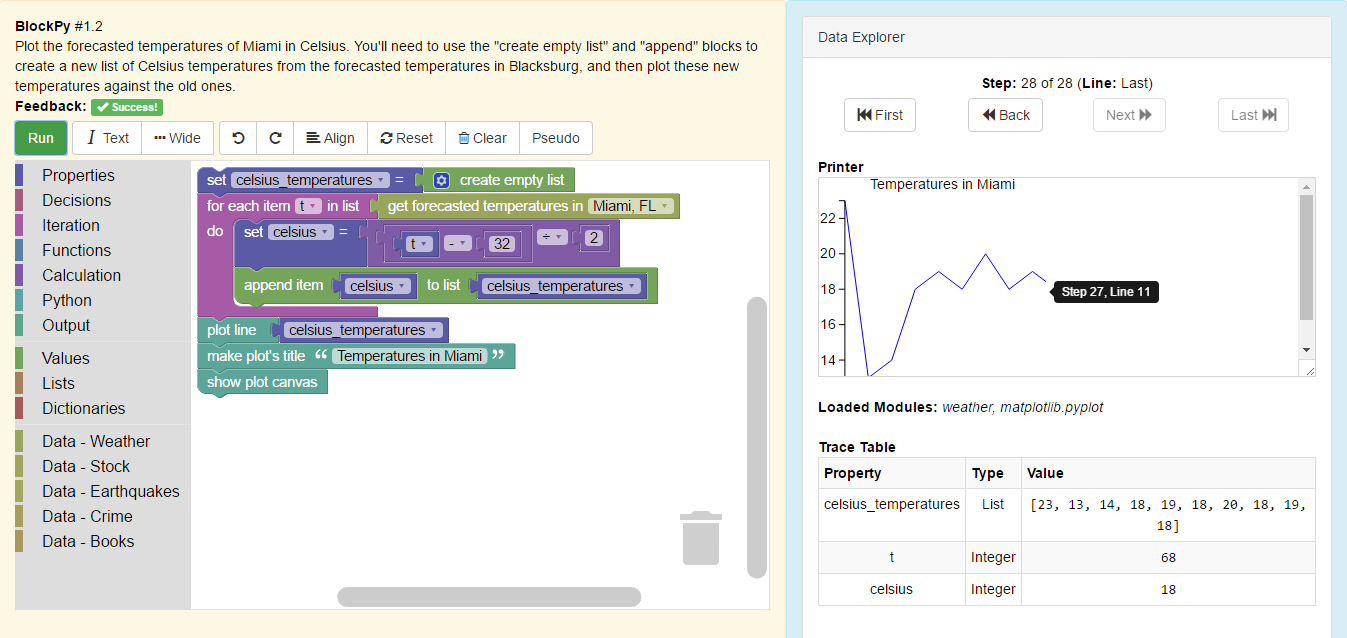
\includegraphics[width=\textwidth]{images/blockpy-screenshot}
\vspace{-\medskipamount}
\vspace{-\bigskipamount}
\caption{A Screenshot of BlockPy in Action}
\label{fig:blockpy-screenshot}
\vspace{-\medskipamount}
\end{figure*}


\section{\textit{BlockPy}'s Major Features}

In this section, we describe the major features of BlockPy.
We view the contribution of BlockPy as the synthesis of known features that are carefully integrated into an environment of novice learners, within the technical constraints of client-side execution.
An overview of the web-based interface is shown in Figure~\ref{fig:blockpy-screenshot}.
At a high level, the left side of the interface is the editor, and the right side is where code execution and output is visualized.
%The goal of BlockPy is to make itself unnecessary, and graduate the learner into a professional programming environment.
%Scaffolding eases this transition and, where possible, the environment attempts to maintain an authentic programming experience.
%Figure~\ref{fig:blockpy-screenshot} shows the version of BlockPy used in the associated study, while recent versions change some of the layout.

At a high level, the left side of the interface is the editor, and the right side is where code execution and output is visualized. The editor area has a menu on the left from which blocks can be selected and a canvas for composing the blocks to create a program. The menu items beginning with ``Data'' expose blocks for accessing data in the CORGIS library. The editor area also contains a row of buttons. The ``Run'' button initiates a browser-based execution of the program. The ``Text'' button controls the dual block/text modes. The ``Pseudo'' button displays a pop-up window with a natural language description of the program. Immediately above the row of buttons is the ``Feedback'' label next to which guided feedback is displayed. In Figure~\ref{fig:blockpy-screenshot}, the guided feedback is the word ``Success'' indicating that the program is correct according to the instructor-authored checks for this problem. The area on the right labeled ``Printer'' displays the program's output. In Figure~\ref{fig:blockpy-screenshot}, a line graph produced by the program is shown. The buttons at the top (``First'', ``Back'', etc.) control the property explorer whose information is displayed in the ``Trace table'' at the bottom.

\begin{figure*}[h]
    \centering
    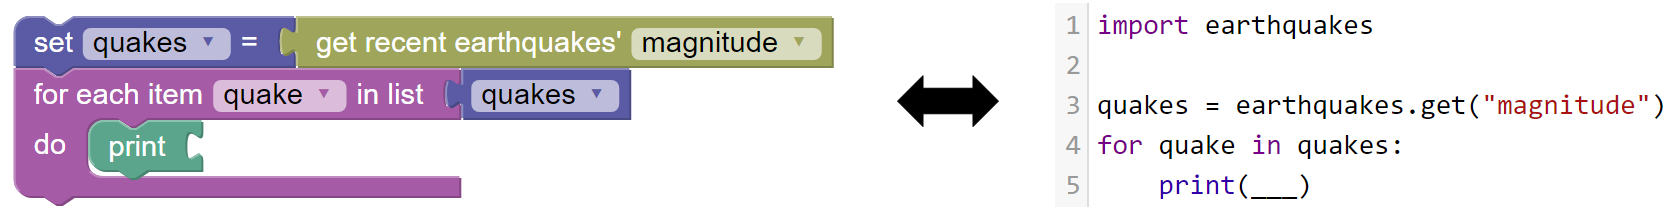
\includegraphics[width=\textwidth]{hq-images/hq_mlt.png}
    \vspace{-\bigskipamount}
	\vspace{-\bigskipamount}
    \caption{Mutual Language Translation between Block and Text interfaces}
    \label{fig:blockpy-mlt}
    \vspace{-\medskipamount}
\end{figure*}

\medskip
\textbf{Dual Block/Text Modes}
One of the most visible features of BlockPy is its dual text/block interface.
At any time, users can switch between a block or a text representation of their code, as shown in Figure~\ref{fig:blockpy-mlt}.
The dual block/text mode is an important scaffold, gradually allowing the learner to move from a supportive block environment to a more professional text-based programming environment. Our experience with university-level non-computer science majors is that scaffolding of this kind is important. 
The block interface uses the Google Blockly library~\cite{fraser2013blockly}, while the text interface uses the CodeMirror library~\cite{haverbeke2011codemirror}.
The Blockly library has been extended with a number of new blocks and features to connect more gracefully with the Skulpt execution engine.
In particular, Skulpt parse trees can be converted into Blockly parse trees.

\begin{figure}[!h]
    \centering
    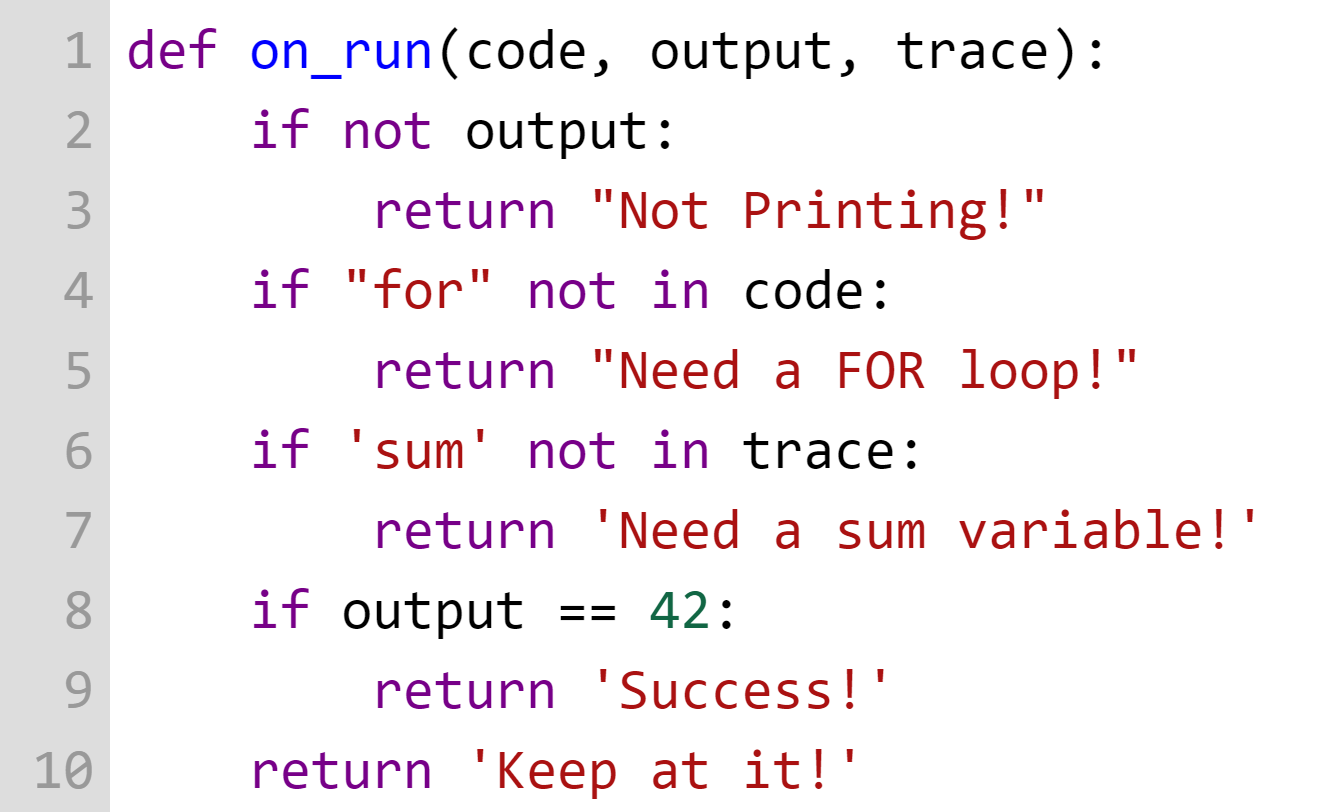
\includegraphics[width=2.6in]{hq-images/hq_instructor_code.png}
    \vspace{-\medskipamount}
    \caption{Example of Instructor-written Guided Feedback code}
    \label{fig:guided-feedback-code}
    \vspace{-\medskipamount}
\end{figure}

\medskip
\textbf{Guided Feedback}
Another valuable pedagogical component of BlockPy is its Guided Feedback system.
% Through a custom interface, instructors define a function that takes the student's code, a trace of its execution, and any output; the function can then return HTML feedback or an indication that they have completed the problem.
% An example of this definition is shown in Figure \ref{fig:guided-feedback-code}.
% BlockPy is able to give many kinds of guidance, controllable by the instructor: suggestions on what is wrong, hints on what to fix, specific instructions to seek further help, or even complimentary feedback.
% For example, in a problem where students must sum a list of integers representing temperatures, the instructor can write feedback code to detect the presence of a \texttt{FOR} loop in the code---if it is not present, then a message could be displayed suggesting they need to read a chapter about Iteration.
% BlockPy's regular error messages have been extended with additional information for beginners.
As shown in Figure \ref{fig:guided-feedback-code}, instructors define a function taking the student’s code, a trace of its execution, and any output produced.
When the program is run the function is automatically executed and can return feedback or an indication that the output is correct.
By combining static and run-time information the feedback code can provide many kinds of guidance: suggestions on what is wrong, hints on what to
fix, helpful readings, or even complimentary feedback.
For example, in a problem to sum a list of integers, a student could be informed that the iteration statement is not properly formed, that an initialization is missing, or that a given section of the textbook is relevant.
Complimentary feedback can sustain the student's motivation and help avoid misguided changes to correct parts of the program.
The desire of students for informative feedback and the extensible nature of the feedback mechanism motivates improvements described in the future work.

\medskip
\textbf{Python Execution Environment}
BlockPy uses the Skulpt engine to execute Python code entirely within the users' browser.
Skulpt works as a ``transpiler'', or source-to-source compiler.
It parses a string of valid Python source code into an Abstract Syntax Tree represented as a JSON-encoded object.
A symbol table is constructed, and then a JavaScript execution engine interprets the AST.
No bytecode is created, and the JavaScript is executed within the client's browser.
Skulpt uses suspensions so that code execution is a non-blocking activity.

The biggest advantage of this approach is that code can be executed much faster since there is no round trip to a server.
Students can continue to work without an Internet connection.
Complicated sandboxes are unnecessary for running the student's code, since they are limited to the API exposed by their browser.
In fact, Skulpt even protects the client's environment, since the Window namespace is hidden.

\medskip
\textbf{Natural Language Code Description}
Another scaffold of BlockPy is a natural language program description generator.
Conventionally, written code is parsed into an Abstract Syntax Tree.
In BlockPy, the transition occurs in the other direction---an AST is used to generate a string of conventional English text.
It can be seen as a third phase to the existing dual text/block mode, although it does not support editing, being a one-way transition.
The goal of this code explanation is for students to better understand the meaning of their code.
Obtuse language features can be translated into more meaningful statements.

\medskip
\textbf{Property Explorer}
After a program is run, BlockPy supports traversal of the executions' trace.
We have found through classroom observations that introductory students often struggle to trace the execution of their programs on their own.
Using the property explorer, not only can students observe the appearance and value of their variables, but also their type.
Further, they can ``rewind'' print and plot operations to observe the impact of these statements.

%\medskip
%\textbf{Parson's Problems}
%Parson's Problems are an example of how scaffolding can help a student solve a problem~\cite{parsons2006parson}, and are available as an optional mode for a problem.
%When a problem is in Parsons mode, all or most of the blocks needed are provided.
%These blocks will be out of order, disconnected, or otherwise incomplete.
%The block editor will randomly shuffle the location of blocks, but it will not break their overall ordering; if statement A comes before statement B, then block A will always be above block B.

\medskip
\textbf{CORGIS Integration}
BlockPy promotes a data science learning context by natively integrating CORGIS.
CORGIS contains diverse data, from authoritative sources.
The subset of CORGIS exposed in the current BlockPy interface is selected based on perceived popular appeal, simplicity, and pedagogical affordances of the data.
These libraries are available through simple blocks.
These blocks translate into function calls that return structured data at varying levels of complexity depending on the block chosen (e.g., \texttt{get\_temperature} returns a single integer, \texttt{get\_temperatures} returns a list of integers, \texttt{get\_forecasts} returns a list of dictionaries with integers and strings, etc).
Figures~\ref{fig:blockpy-screenshot} and \ref{fig:blockpy-mlt} demonstrate these blocks in use.

\medskip
\textbf{Plotting}
Another addition to Skulpt is tools for making visualizations, a core activity for data science.
Currently, BlockPy supports the creation of line plots, scatter plots, and histograms using an API identical to the popular MatPlotLib API.%~\footnote{http://matplotlib.org/}.%~\cite{SkulptMatPlotLib}.
By mimicking this professional API, BlockPy increases authenticity and promotes transfer.
Students in our course, for example, transfer this learning to their final projects where they use MatPlotLib from the Python program they write.



\medskip
\textbf{LTI Support}
Although BlockPy has its own internal course management system, it also supports LTI (Learning Technology Interoperability). 
%This important standard separates ``Tool Consumers'' from ``Tool Providers''.
That is, it provides a mechanism for Learning Management Systems (e.g., Canvas, Sakai, Blackboard, Moodle) to interact with external tools.
Instructors who have configured BlockPy to work with their LMS can select, create, and edit assignments all from within their LMS of choice.
When students complete problems in the BlockPy environment, they are automatically graded, and the LMS is given the relevant information.

LTI supports user authentication through Canvas (and potentially other LMS).
When a student loads a BlockPy problem, Canvas delivers their email address to BlockPy.
This information is used to determine if an account exists for that student.
If it does not, they are introduced to the system and vouched for by the LMS.

%To support the LTI standard, we have started work on spinning off a template for future Python-based LTI applications.
%This open-source project is available at \url{https://github.com/acbart/lti-flask-skeleton}.

%\medskip
%\textbf{Dangling Blocks}
%The block editor allows users to create statements that are not fully formed or connected.
%At any given time, blocks may be disconnected.
%This is consistent with BlockPy's design philosophy of incremental development.
%When a student transitions from blocks to text, unspecified expressions are converted to quadruple underscores, and unspecified statements are converted to empty ``pass'' statements.

%\medskip
%\textbf{Free and Open-source}
%Consistent with the open-access nature of BlockPy, the entire project is free and open-source.
%We do not present BlockPy as a finished product, but merely another step in the development of educational tools for teaching introductory programming.
%We anticipate that features of BlockPy have value to other introductory environments.
%Making its source code freely and readily available is an important step in promoting our vision.


\section{Design Issues}

We next present design issues that were encountered when developing BlockPy.
These issues should be of interest to developers of introductory environments.

\subsection{Internal Code Representation}

Dual block/text editors create an added challenge in deciding the right internal representation of the students' code.
BlockPy uses the textual version as the canonical representation, as opposed to the block parse tree.
This choice facilitates the text mode display and program execution. 
However, there were other options.
Some editors operate on Parse Trees exclusively.
Others treat the source code as a list of lines (separating elements by the newline), sometimes attaching special properties to individual lines such as geometric information~\cite{Bau}.
A major limitation of both representations is that some valuable programmer-level semantic data is not preserved.
On the text side, user-created whitespace does not survive the transition.
On the block side, block layouts are reset according to the default rules.
The original dual text/block editor created by Mastuwaza~\cite{Matsuzawa} solved this problem by storing geometric information of blocks in the comments of the text mode.
However, this leads to crowded code with confusing comments.
The trade-offs in Mastuwaza's system led to BlockPy's design as a primarily text-driven environment.

\subsection{Block Language}

A criticism of the block interface is that the blocks do not use accurate Python syntax.
For example, the collection iteration block that models a Python \texttt{for ... in} loop has plain text phrasing, to explain the nature of the block more clearly: \texttt{for each item [\_\_] in list [\_\_]}.
Similarly, the assignment block has the text \texttt{set [\_\_] = [\_\_]}.
Over time, BlockPy's exact wording has evolved to more closely match Python.
However, we feel that explicit text is more helpful to beginners.
Although there are advantages to more understandable blocks, there are credible concerns that beginners may learn incorrect syntax.
We comment further on this in Section 5.3.

%There are many cases to consider when designing a block language:
%Should equivalence testing (equal to, not equal to, greater than, etc.) use common math symbols or correct Python code?
%Should the function declaration block use the \texttt{def} keyword or the more accessible word \texttt{define}?
%Square brackets (\texttt{[]}) indicate an empty list in Python---is that more obtuse than the phrase \texttt{create empty list}?
%In Section~\ref{sec:Evaluation}, we analyze preliminary empirical data about the subject.

%\subsection{Block Hiding}

%An advantage of Python as a teaching language is the terseness of its grammar.
%The simplest ``Hello World'' program in Java, for example, requires the explanation or hand-waving of a half-dozen keywords and symbols: ``\texttt{public}'', ``\texttt{static}'', ``\texttt{void}'', etc.
%In Python, a single statement or expression can be used to print, depending on the environment.
% However, Python is still a language with syntax and order, and so certain commands are necessarily complex.
% This is not a criticism of the language, but an observation that perfectly reasonable tasks may have hidden pedagogical costs.
% In particular, the data science approach we take with BlockPy demands that students import modules in order to gain access to the data methods.
% In Python, this translates to an \texttt{import} statement and a method call on the imported module.

% The goal of the data science context is to minimize the secondary pedagogical requirements that may distract from primary learning objectives.
% Therefore, in the BlockPy interface, import statements are not rendered directly in the block interface, but are present in the text view.
% Obvious alternatives include creating special \texttt{import} blocks that appear on demand, or a special notification within the interface that an external library is being used.
% Both approaches necessitate discussion of code importing.

% A major disadvantage of hiding the imported module is that the module name still enters into the program's namespace.
% This means that students may end up choosing reasonable variable names that collide with modules that they unknowingly use.
% Figure~\ref{fig-degenerate-code} demonstrates code that extracts data from a module and then overwrites the module's variable with that data.
% Although this does not have any impact on the syntactical or semantic execution of the code, the code becomes misleading.
% Alternative names could be used to prevent namespace collisions, such as \texttt{weather\_module} or \texttt{stocks\_data\_source}.



\subsection{Parser Errors vs. Syntax Errors}

In theory, it is impossible to generate syntactically incorrect Python code when transitioning from the blocks to text.
However, it is quite possible for students to write invalid code in the text mode, making the transition back to blocks problematic.
A missing colon, unclosed parentheses, or incorrect indentation will prevent Skulpt from generating a valid parse tree.
When encountering code with a syntax error, BlockPy creates ``raw blocks'' that store the literal Python code.
BlockPy will also create raw blocks for language features that are not implemented in the block interface, but most of these features are uncommon, such as \texttt{else} bodies in \texttt{for} loops.

The algorithm for translating code attempts to create as many blocks as possible, but can often be confounded into creating one large raw block.
Although some might consider this a disadvantage, it is not necessarily desirable to ensure that students always write completely valid programs at all times, especially in the early stages of constructing an algorithm or when new programming constructs are introduced.
Although BlockPy is built on the premise that it is worth delaying the conversation about syntax, students must eventually become comfortable with the details of writing syntactically correct text code.

It is not always possible to automatically correct a students' written code to match their intent.
(Sometimes students may not even understand their own intent!)
However, there are more sophisticated approaches to improving the support given to students.
A more robust parser could be developed to precisely identify student code errors.
Alternatively, every subset of the code could be parsed in isolation in order to determine what areas of the code are correct.
%Rivers and Koedinger explore other approaches that uses prior student submissions for each problem to suggest corrections to the user~\cite{rivers2015data}.

\section{Evaluation of BlockPy}
\label{sec:Evaluation}

We now describe the results of a deployment of BlockPy.
BlockPy has been used in an introductory Computational Thinking course for four semesters.
This course is meant for non-Computer Science majors from the humanities, arts, and the sciences.
They typically have no prior programming experience and have a limited understanding of the field. 
Therefore, they ideally model the anticipated BlockPy user.

\subsection{Methodology}

\begin{table}[!h]
\renewcommand{\arraystretch}{1.3}
\caption{Overview of the BlockPy Curriculum}
\label{table:blockpy-curriculum}
\centering
\begin{tabular}{l|c|c}

Problems & Type & Topics \\\hline
\#1.1-\#1.5 & Classwork & Printing, Variables, Plotting\\\hline
\#1.6-\#1.8 & Homework & Printing, Variables, Plotting\\\hline
\#2.1-\#2.5 & Classwork & Iteration, Accumulation, Mapping\\\hline
\#2.6-\#2.8 & Homework & Iteration, Accumulation, Mapping\\\hline
\#3.1-\#3.6 & Classwork & Conditionals, Filtering Lists\\\hline
\#3.7-\#3.8 & Homework & Conditionals, Filtering Lists\\\hline
\#4.1-\#4.6 & Classwork & Textual Code, List Transformation\\\hline
\#4.7-\#4.A & Homework & Textual Code, List Transformation\\\hline
\end{tabular}
\end{table}

In the Spring 2016 offering, 50 students were assigned 34 BlockPy problems over the course of 4 classes over 2 weeks (see Table~\ref{table:blockpy-curriculum}).
This focused use of block programming built upon their notions of algorithms, which they had previously seen during a 6-week introductory unit where students created algorithms using natural language and flowcharts.
Most of the problems were assigned as classwork, with the expectation that any incomplete assignments were to be done as homework.
Typically, classwork problems would give students starting code.
Homework questions would have them complete similar problems from scratch.
After the BlockPy unit, the curriculum continued in the Spyder IDE, a more conventional desktop programming environment.
To facilitate this transition, the last day of BlockPy material started in text mode, and encouraged students to become familiar with writing code in that form.
BlockPy was not intended to be used for all programming in our course, and was faded in the transition to Python.
In contrast to other curricula~\cite{mediated-alice}, for our college-level learners, the BlockPy scaffolding could be removed after 4 days.
More information about the curriculum can be found in~\cite{kafura2015design}, and at the course's public site~\footnote{\url{https://think.cs.vt.edu/course_materials/}}.

\begin{figure}[!h]
    \centering
    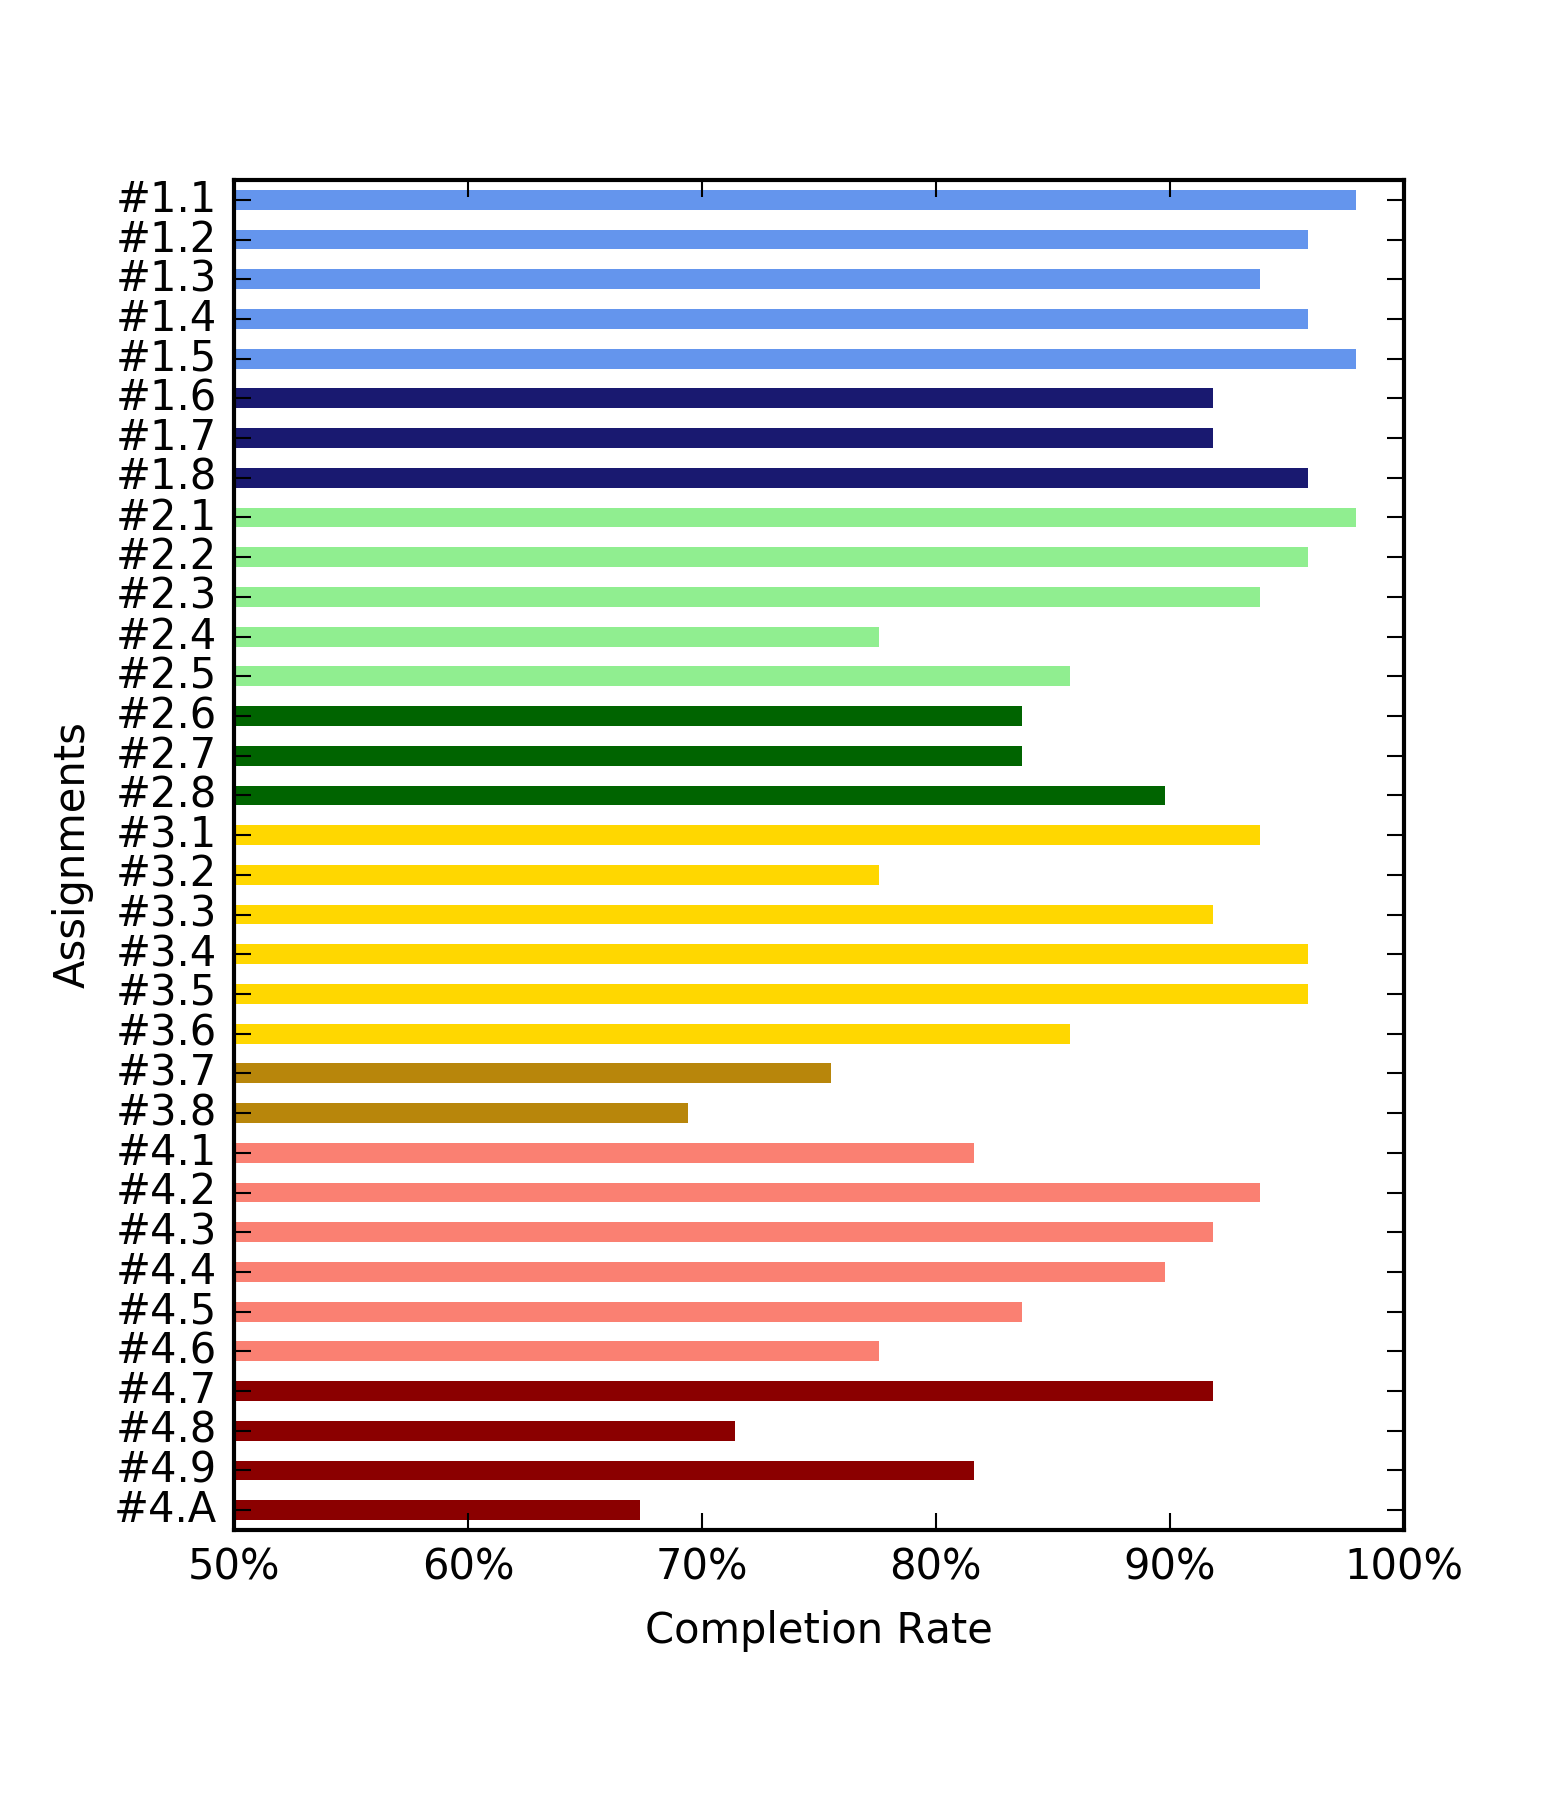
\includegraphics[width=\columnwidth]{hq-images/hq_smaller_successes.png}
    \vspace{-\bigskipamount}
    \vspace{-\bigskipamount}
    \vspace{-\medskipamount}
    \caption{Completion Rate by Problem (colors indicate distinct days, brightness indicates homework vs classwork)}
    \label{fig:success-over-problems}
    \vspace{-\medskipamount}
\end{figure}

\begin{figure}[!h]
    \centering
    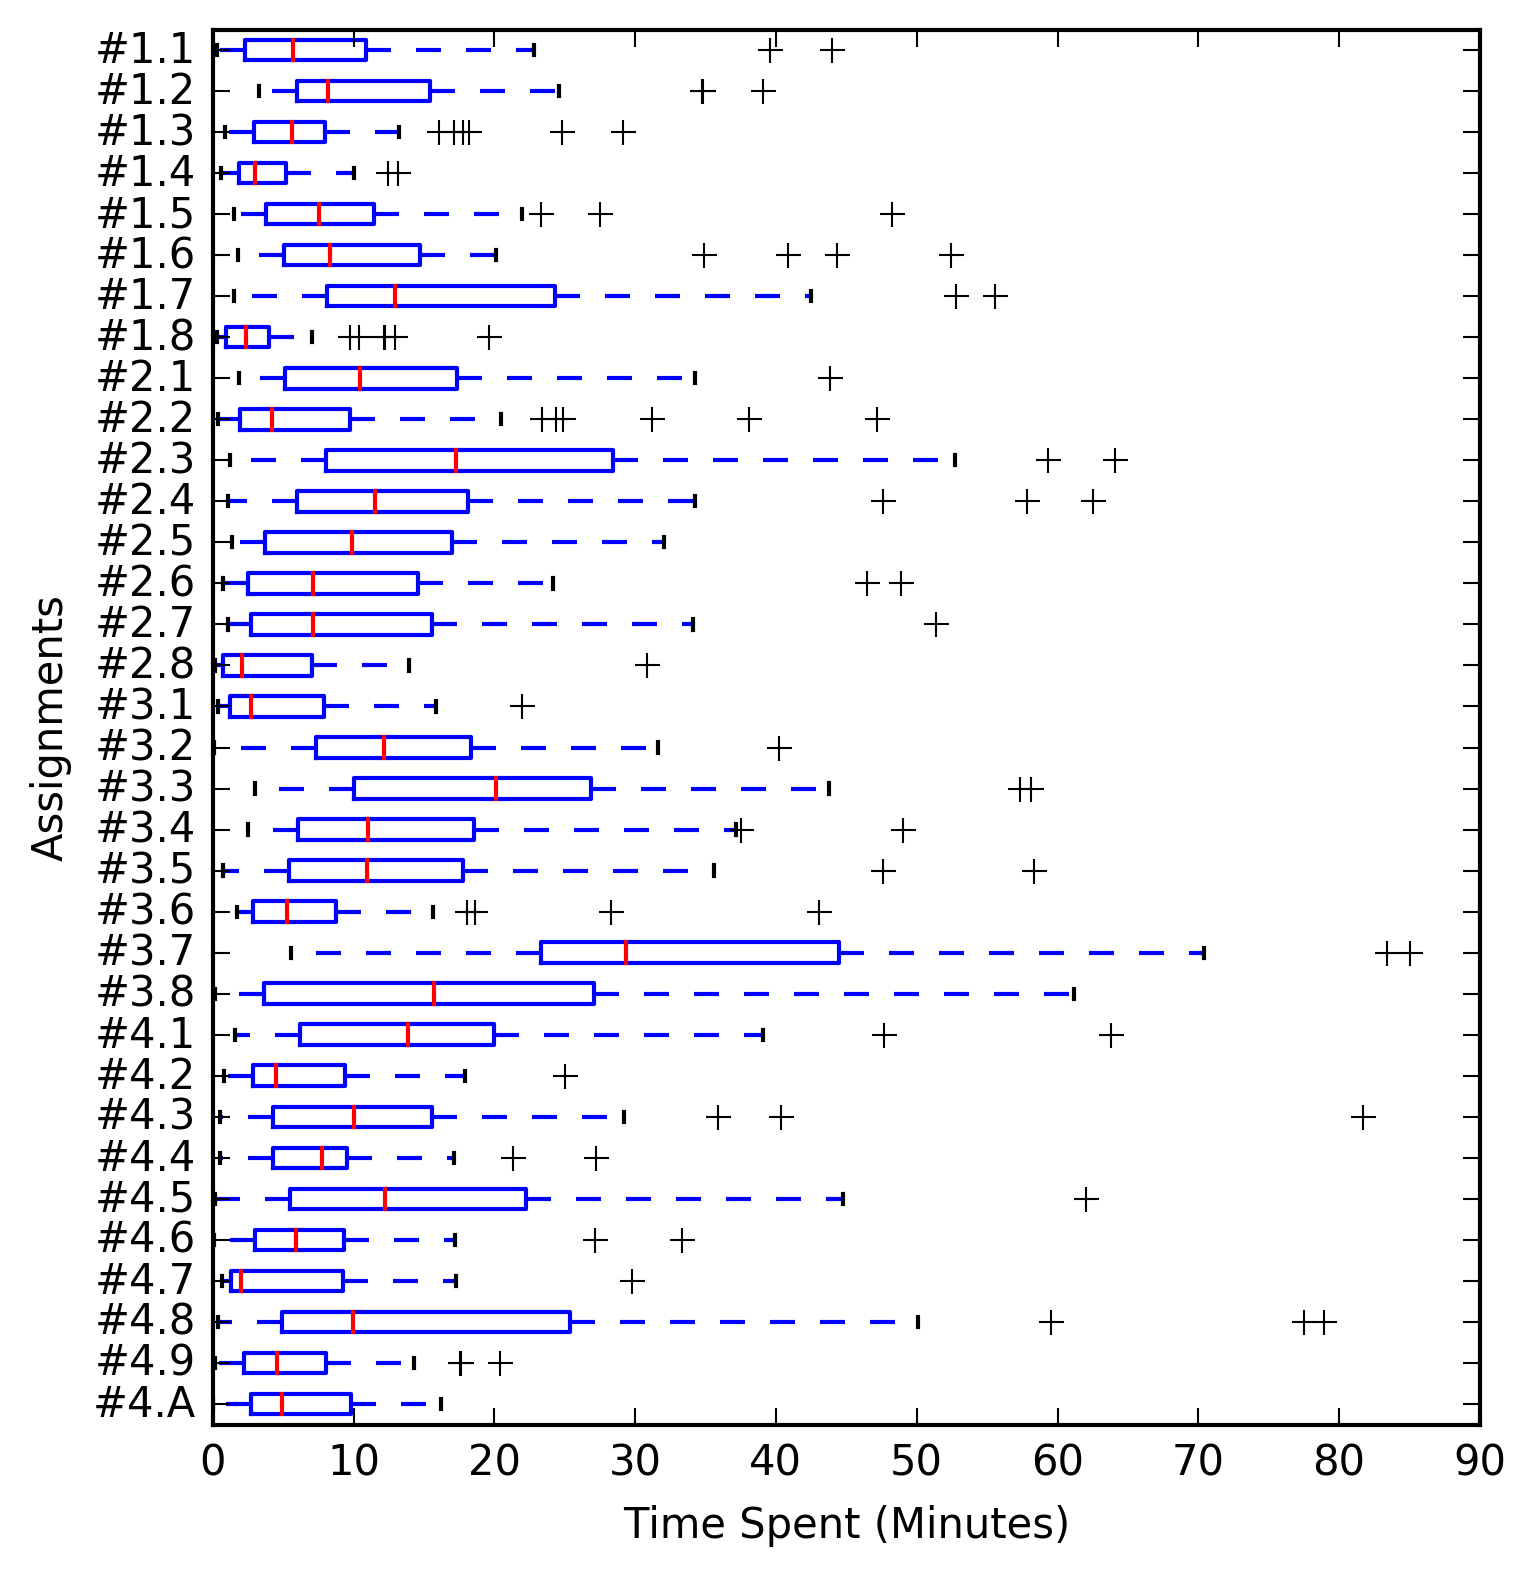
\includegraphics[width=\columnwidth]{hq-images/hq_smaller_worksession_length.png}
    \vspace{-\bigskipamount}
    \vspace{-\medskipamount}
    \caption{Work Session Length (minutes) by Problem}
    \label{fig:total-session-length}
\end{figure}

Figure~\ref{fig:success-over-problems} describes student completion rates over the assignments.
The bars are colored to indicate day (there were four days of BlockPy activities), and their brightness indicates homework vs. classwork.
Figure~\ref{fig:total-session-length} describes the distribution of time spent on each problem.
92\% of the 50 students completed more than 60\% of the 34 problems and 62\% of the students completed more than 90\% of the problems.
The average student was able to complete most problems in 15 minutes, which was considered reasonable by the instructors.

% While these aggregate results are positive, we found deficiencies with specific problems.
% Some seemed to take students much longer than anticipated, such as \#3.7, which had students write code from scratch to identify the index of the minimum value in a list.
% As students progressed through the curriculum, there is a visible reduction in the percentage of completions.
% There is a similar reduction from classwork to homework.
% While the completion rate almost always remains above 70\%, there was a noticeable drop-off on the last day.
% This is most likely caused by three things: fatigue on the part of the students (accumulated work load might have been overwhelming), the proximity to the end of the unit (which means that students had comparatively less time to work on these problems than earlier problems), and the fact that Day 4 is the transition to text mode and students struggle with the new syntax.

BlockPy evaluation is based on two data sources.
First, fine-grained logs were collected of the students' interactions with BlockPy, including any changes made to their code at the keystroke/block level and interface actions.
Second, a survey was administered 2 weeks after BlockPy was completed.
41 out of 50 students gave consent for their answers to be released for research purposes, with 
19 male students and 22 female students.
32\% were freshmen, 39\% were sophomores, 17\% were juniors, and 12\% were seniors.

This survey had four free-response questions asking students about frustrating and helpful features in both BlockPy and Spyder:\\\indent
1) What features of BlockPy were most helpful?\\\indent
2) What features of BlockPy were most frustrating?\\\indent
3) What features of Spyder were most helpful?\\\indent
4) What features of Spyder were most frustrating?

We performed qualitative, open coding on the free response questions, converging on a set of generalized tags.
42 students responded to each of the 4 questions.
The responses were brief phrases and sentences, with only a scant few having more than one sentence.
One author was tasked with performing the open-coding on the survey responses in order to find general tags; each response was first condensed into a brief specific tag, and then common tags were grouped into more general clusters.
For example, for the Frustrating BlockPy features question, there were 42 responses which were generalized into 21 specific tags, which were in turn generalized further into 10 tags.
Table \ref{table:blockpy-survey-qualitative} presents the generalized tags gathered during the qualitative coding.
The tags are grouped by the Features column, which identifies which environment students were responding to and whether they were considering its helpful or frustrating aspects.
The number of occurrences of each tag across student responses is given in the third column.
Only tags with 5+ occurrences were included.
Sections 5.2 and 5.4 describe the results of this analysis.

The survey asked this multiple-choice question about where students felt the BlockPy/Spyder transition should occur:
``When do you think we should have STOPPED using BlockPy and started using Spyder?''
In addition to an ``Other'' response, six alternatives were given: the three choices ``Always'', ``Never'', ``The Same'', and and three different places in the curriculum, implying more or less use of BlockPy.
The results of this question are discussed in Section 5.3.

\begin{table}[!t]
\renewcommand{\arraystretch}{1.3}
\caption{BlockPy Survey Qualitative Results}
\label{table:blockpy-survey-qualitative}
\centering
\begin{tabular}{c|c|c}
\hline
Features & Generalized Tag & N (\%)\\\hline
Helpful BlockPy & Block Interface & 24 (57.1\%) \\
 & Dual Text/Block & 12 (28.6\%)\\
& Guidance & 5 (11.9\%)\\\hline
Frustrating BlockPy & Vague Guidance & 19 (45.2\%)\\
  & Block Interface & 7 (16.7\%)\\
  & Programming & 5 (11.9\%)\\\hline
Helpful Spyder & Better errors & 16 (38.1\%)\\
& Variable Explorer & 17 (40.5\%)\\
& Writing text code & 5 (11.9\%)\\\hline
Frustrating Spyder & Error Messages & 12 (28.6\%)\\
& Text Coding & 7 (16.6\%)\\
& Interface & 6 (14.3\%)\\
& Crashing & 5 (11.9\%)

\end{tabular}
\end{table}

%\item The effectiveness of the scaffolded learning environment, % (interface has merit + dual text/block interface, misleading blocks)
	%\item Novice learners didn’t use most of the interface% (Tool use in BlockPy)
    %\item Improved feedback is needed% (improved guidance + static analysis)
    
\subsection{BlockPy's Helpfulness}
%\subsection{The Interface has Merits}

\textit{Do novice learners find the BlockPy features helpful?}

To answer this primary research question, the results of the survey were analyzed for commonly repeated sentiments by students.
Students gave positive responses about BlockPy's block interface.
57\% indicated the block interface as particularly helpful.
Two representative responses are:

\textit{``You could much more easily visualize the code, and you didn't have to worry about grammar and the text language.''}

\textit{``That we didn't have to write the code and worry about indentation, punctuation.''}

29\% indicated that the dual text/block interface helped. For example:

\textit{``I liked the ability to switch between text code and the blocks''}

\textit{``Being able to switch from text to block view. Even after we stopped using BlockPy I could put my code into it and it helped me [see] where I was wrong''}

Taken together, this feedback, comprising 85\% of the students, suggests that the highly visible block interface is what students find most helpful in BlockPy.

Only 12\% found that the guidance offered by the feedback mechanism particularly helpful:

\textit{``... I found it helpful when there was information to guide me when I could not proceed and obtain the correct answer.''}

\textit{``... I also liked that it would give hints and tell you when the code was correct.... ''}

In terms of frustrations, 19\% of the students found the guidance provided by the automatic feedback mechanisms to be vague. This issue is discussed further in Section 5.4. While the block interface was generally well received, 


\textit{``Making the blocks link up in the way I wanted was kind of finicky sometimes.''}

\textit{``the constant dragging of blocks.''}


Other frustrations were with the problems assigned or the nature of coding in general.

\textit{``everything when you can't figure out how to successful run the program''}


Helpful features of Spyder included better error reporting and the variable explorer feature. While the feedback in BlockPy was criticized by 45\% of the students, 38\% found the feedback in Spyder helpful. While both BlockPy and Spyder included a variable explorer feature (to display the values of variables during and after execution), this feature was mentioned positively by 40\% of the students. The positive view of this feature in Spyder may be due the greater need for a variable explorer in the text programming part of the course which introduced more complex data structures.
Comparatively, many criticisms of Spyder related to coding in general, rather than features of the environment (e.g., students described frustrations with Python syntax, trying to interpret errors).


\textit{``Very small details that are inherent in coding. Things like capitalization and other very small details were annoying...''}

\textit{``None. Writing code in general is frustrating.''}

\subsection{Evaluation of the Scaffolds}

\textit{Is the BlockPy scaffolding effective in transitioning novice learners from a block-based environment to a professional text environment?}

\begin{figure}[!h]
    \centering
    \vspace{-\medskipamount}
    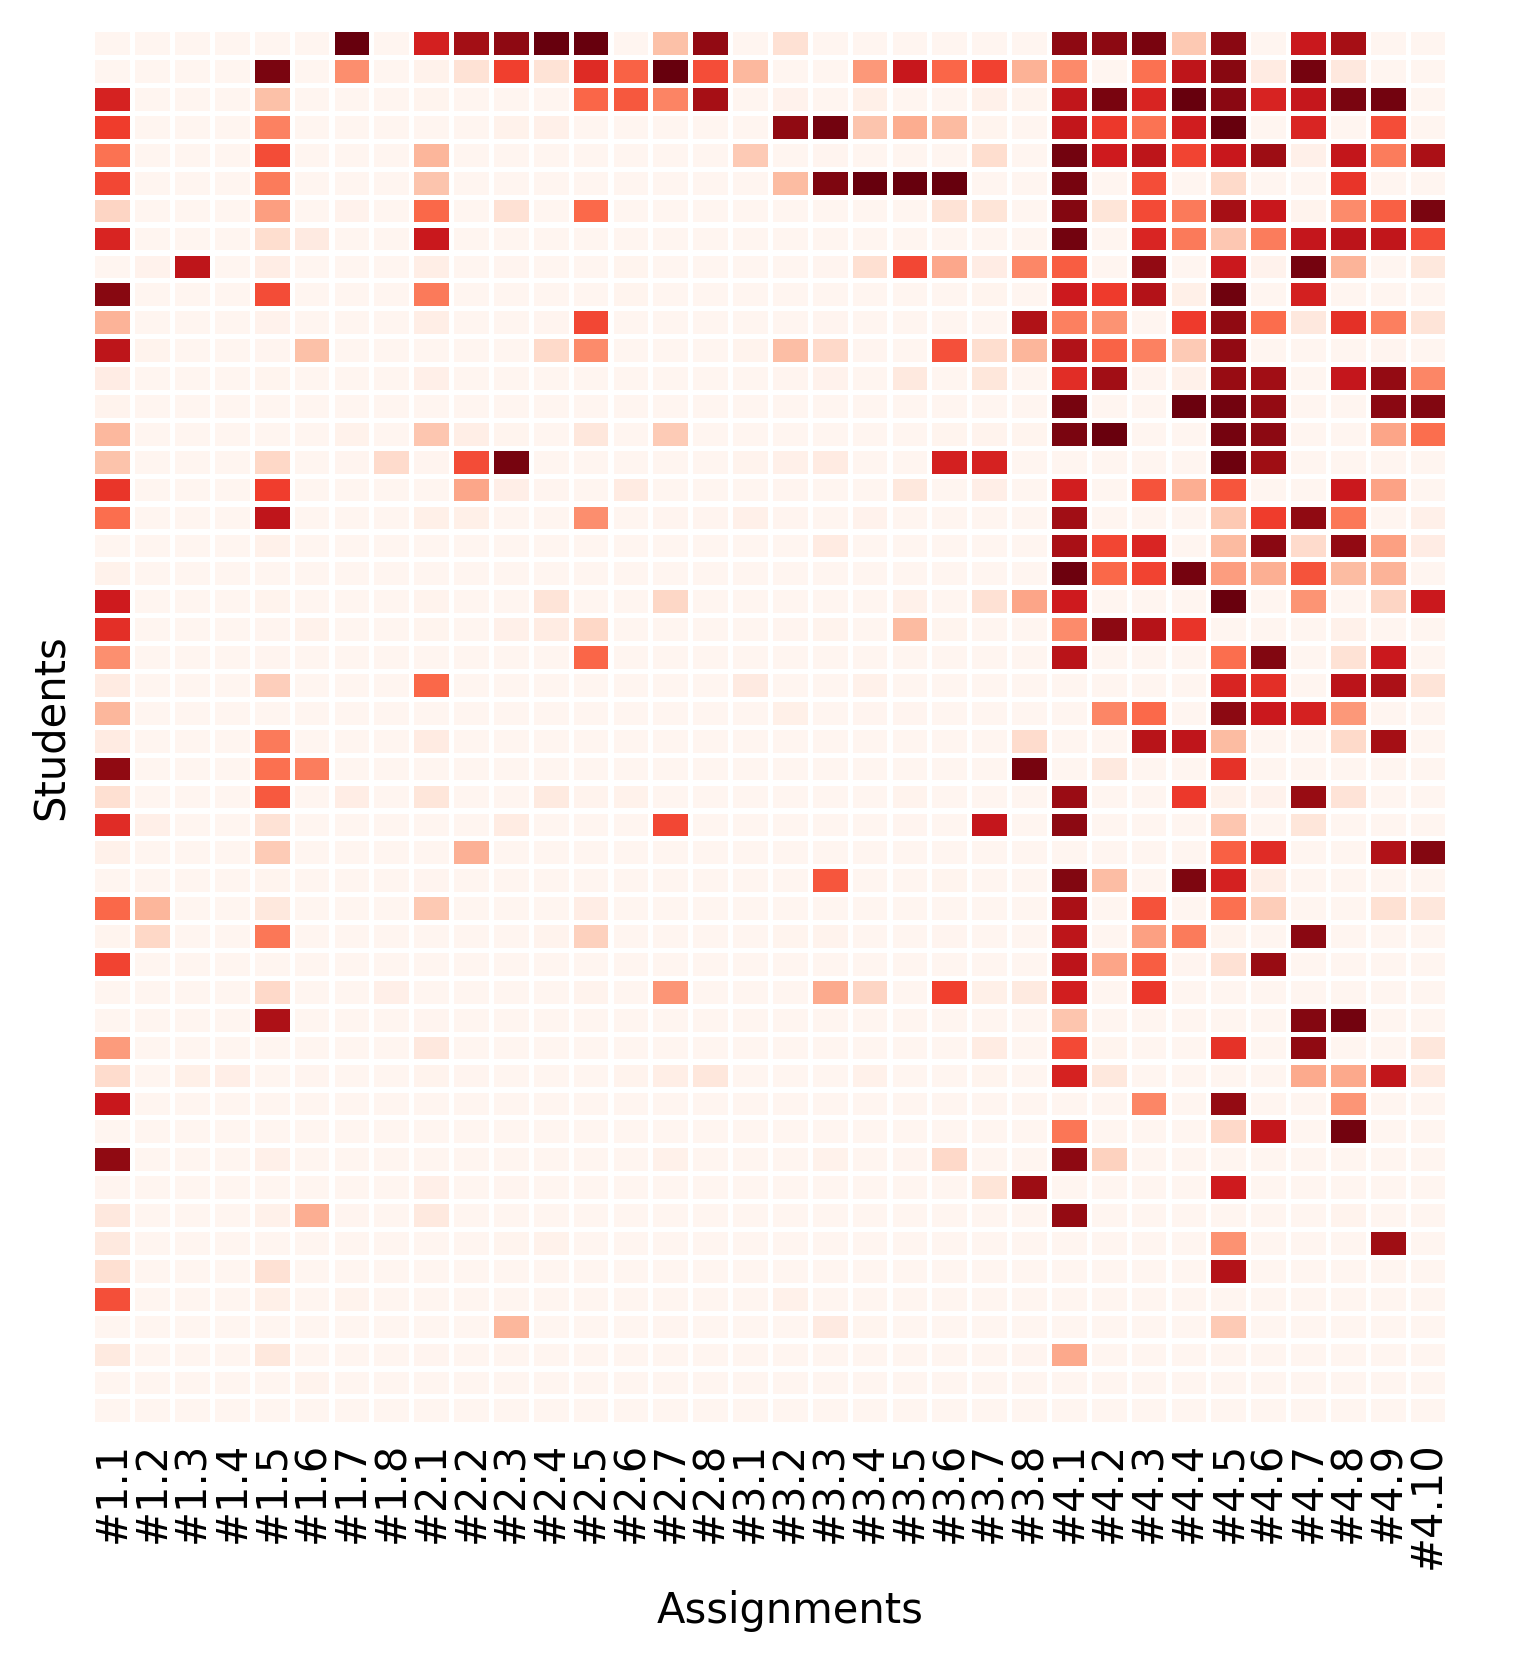
\includegraphics[width=\columnwidth]{hq-images/mode_heatmap.png}
    \vspace{-\bigskipamount}
    \vspace{-\medskipamount}
	\caption{Time Spent in Text-mode by Students on each Assignment}
    \label{fig:time-spent-mode}
    \vspace{-\medskipamount}
\end{figure}

To answer this question we analyzed various aspects of the students use of the dual block/text feature of BlockPy, particularly during the transition from BlockPy to the text-only Spyder IDE.
Figure \ref{fig:time-spent-mode} is a grid-based representation of students' time spent in text mode while working on assignments, with redder cells indicating more time spent in text mode.
Each row of cells represents another students' progression through the assignments, given on the X-axis.
For the first 3 days of the assignments, students mostly stayed in the block interface (with the first problem being a notable exception, since it was used to show students how the interface was dual-block/text).
It is encouraging to note that some students did switch between the block and text editor in several early problems, if only to observe the resulting code.
However, it is also clear that many students stayed almost entirely in the block mode, even during the final problems.
This graph does suggest that more incentives and guidance could be given to direct students to pay attention or take advantage of the text interface when the problem expects them to, to build their competency with that form of their programs.
It is interesting to note that there are a small number of students who used the text mode almost exclusively; anecdotally, some students expressed that they found the text interface more understandable than the block interface.
It is another advantage of the dual block/text interface that both kinds of students, those who prefer blocks and those who prefer text, can use the system without issue.

The last day of BlockPy began the transition to full textual Python programming.
Students tended to spend more of the last day in the text interface, which was encouraged by the interface starting in text mode and the problems asking students to write their programs in text rather than blocks where possible.
To prepare students for the transition, they are given a translation guide showing individual blocks and their equivalent textual form in Python.
The day's lecture covered basic text syntax, and gave side-by-side examples of blocks versus Python text.

%%% Misleading Blocks
One effect observed in the transition to text was that students were confused by the difference in keywords between BlockPy and Python.
As previously described, the keyword text on blocks is often more verbose than the actual Python syntax.
This is intended as a feature to improve learners' understanding of the blocks.
However, analysis of the logs suggest that this causes confusion for some students when they transition to writing text code.
A crucial question is how wide-spread this problem is and how long it persists.
We looked at three types of mistakes that students could make due to the keyword differences: writing \texttt{for each X in Y} instead of \texttt{for X in Y}, writing \texttt{set X = ...} instead of \texttt{X = ...}, and writing \texttt{if X then do ...} instead of \texttt{if X}.
We found 20 students who exhibited this behavior in 29 different incidences across all the problems: 9 incorrect \texttt{for}, 17 incorrect \texttt{set}, and 1 incorrect \texttt{if}.
Few students made the mistake on more than one problem.
In over 60\% of the cases, the student corrected their mistake within a minute, and in 23\% the student corrected their mistake in 1-4 minutes.
In the two worst cases, students persisted with the incorrect code for over 5 minutes and 7 minutes.
It is worth pointing out that no student ended the assignment (successfully or not) with any use of the word \texttt{each}, \texttt{set}, or \texttt{do}.
While the degree and persistence of the keyword confusion problem is very limited, it does seem prudent for the guidance to correct students who might be using such incorrect code forms.

%%% BlockPy -> Spyder
The survey asked students where they would prefer to make the transition from BlockPy to Spyder, and allowed to choose from a series of intervals in the course.
The majority (28 students) indicated that the current location was appropriate, 6 students indicated that it should be later, 6 indicated that instruction should be kept in BlockPy, and 7 students indicated that it should be earlier.
This provides justification for the relatively short duration of the BlockPy curriculum compared to subsequent sections of the course---the curriculum is intended to transition students into a more mature environment, and so is not meant to last for too much of the course.

% An interesting result from analysis of the logs is shown in Figure~\ref{fig:edit-distance-rates}.
% Edit distance for each user modification (e.g., keystroke, block deletion/addition, etc.) was calculated and then divided by the amount of time spent in the relevant mode.
% From this, an estimate of how productive students were in the two different modes can be seen.
% The average edit distance was more than twice as high with blocks compared to text, most likely because an action in blocks is usually equivalent to a number of keystrokes in text.
% Although this could easily be different for experts and should be taken with caution, it is an encouraging result for block-based programming advocates.

% \begin{figure}[!t]
%     \centering
%     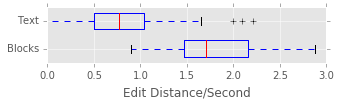
\includegraphics[width=2.5in]{images/edit_distance_mode.png}
%     \vspace{-\bigskipamount}
%     \caption{Edit Distance/Second in Text Mode vs. Block Mode}
%     \label{fig:edit-distance-rates}
% \end{figure}


% \begin{figure}[!t]
%     \centering
%     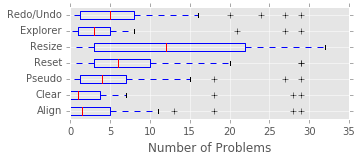
\includegraphics[width=\columnwidth]{images/toolbar_events.png}
%     \vspace{-\bigskipamount}
%     \vspace{-\bigskipamount}
%     \caption{Students' Use of Toolbar Features over Problems}
%     \label{fig:explorer-event-usage}
% \end{figure}

% The main toolbar in BlockPy gives students access to a number of features intended to help them complete problems.
% Some of these tools are standard editor features, such as undo and redo buttons.
% Some of them, however, are more specific to the educational nature of the environment, such as the code explorer and natural language code generator (named \texttt{pseudo} in this version). 
% Figure~\ref{fig:explorer-event-usage} reports on student use of these features across problems.
% Unfortunately, these data suggest that most students did not take advantage of these features.
% Deeper analysis found no significant correlations between student performance (as established by either time on task or number of successfully completed problems) and level of use of the toolbar features.
% The x-axis is the number of problems where a student used the particular feature at least once.
% In part, we attribute this underutilization to these features not being sufficiently emphasized in the instruction.


%\subsection{Managing the Data Science Context}
%\subsection{The State of the Curriculum}


\subsection{Feedback Quality}
\textit{Is the guided feedback effective and sufficient for novice learners?}

To answer this question the free response questions were analyzed.
There was little agreement about what was most frustrating about BlockPy, with one major exception: 45\% of students agreed that BlockPy's automatic guidance could be frustratingly vague.
For example:

\textit{``The hints were not always helpful...they were very ambiguous sometimes which was frustrating.''}

\textit{``The most frustrating part of BlockPy was the tips that it gives you while creating an algorithm because if you were close, it didn't give you more hints as to where specifically the problem is, it just said you still have "a little way to go.''}

This reaction is partially biased by the timing of the survey.
Earlier problems were intentionally equipped with more extensive suggestions and guidance than later problems, so students worked with less helpful problems at the time the students completed the survey.
Regardless, it is clear that students wanted more guidance from the environment.
Giving less guidance in later problems was partially motivated by a desire to have students work more on their own, but was also motivated by the time-intensive nature of developing more sophisticated guidance.

38\% of the students suggested that error reporting in Spyder was more helpful than in BlockPy.
In particular, they typically indicated that being able to identify the exact line that an error occurs in Spyder was tremendously helpful, and a major lack in BlockPy.

\textit{``It was able to tell me exactly what line of code was having an issue and what type of error.''}

Considering that the text mode of BlockPy does have this feature, we believe that students only considered the block interface.
However, it is an understandable concern.
Errors in BlockPy refer to line numbers instead of individual blocks, a disconnect that is recognized by the designers.

\begin{table}[!t]
\renewcommand{\arraystretch}{1.3}
\caption{Incidences of Semantic Errors Detected by Static Analysis of 1587 Student Programs and 1463 Correct Student Programs}
\label{table:static-analysis-errors}
\centering
\begin{tabular}{l|c|c}
\hline
 & All & Correct \\\hline
Changed type of variable & 60.8\% & 62.1\% \\\hline
Variable overwritten without read & 50.9\% & 51.6\%\\\hline
Variable never read & 16.8\% & 14.3\% \\\hline
  Variable read without write & 12.0\% & 9.10\% \\\hline
Iteration list used in iteration & 7.48\% & 6.29\% \\\hline
Iteration variable unused in iteration & 6.53\% & 5.13\% \\\hline
Used iteration list as iteration variable & 6.02\% & 5.88\%\\\hline
Iteration over non-list & 1.58\% & .75\%\\\hline
Used unknown function & .63\% & .63\% \\\hline
Iteration over empty list & .06\% & .07\% \\\hline
%Changed type of variable & 959 & 909\\\hline
%Variable overwritten without read & 803 & 755\\\hline
%Variable never read & 265 & 209 \\\hline
%Variable read without write & 190 & 133 \\\hline
%Iteration list used inside iteration & 118 & 92 \\\hline
%Iteration variable unused inside iteration & 103 & 75 \\\hline
%Used iteration list as iteration variable & 95 & 86\\\hline
%Iteration over non-list & 25 & 11\\\hline
%Used unknown function & 10 & 9 \\\hline
%Iteration over empty list & 1 & 1\\\hline
\end{tabular}
\end{table}

\begin{figure}
\begin{python}
import stocks

stocks = stocks.get_past("FB")
new = []
for stock in new:
    new = []
for stocks in stocks:
    print(stocks)
\end{python}
\vspace{-\medskipamount}
\caption{Degenerate Student Code}
\label{fig-degenerate-code}
\vspace{-\bigskipamount}
\end{figure}

Table~\ref{table:static-analysis-errors} reveals another concern: that students commit many errors that are currently undetected.
The final submission from every student was analyzed using a flow-sensitive static-analysis algorithm that looked for code that, while valid and often matching the problem specifications, exhibited certain degenerative behavior.
In the table, the first column is the type of semantic error, the second column is how many incidences were found in all student programs as a percentage of all programs submitted (50 students over 34 problems submitted 1587 programs), and the third column is how many incidences were found in programs marked correct as a percentage of all programs marked correct (1463 programs submitted that were correct).
Figure~\ref{fig-degenerate-code} gives examples of some of these types of errors: declaring a variable that is never read, reusing the iteration list as the iterator, and in one case even iterating over an empty list.
Often, these errors are silently unreported because they are guarded against by unreachable code paths, or have no impact on the program's output.


\section{Future Work}

We now outline future work and directions for BlockPy.
Some of this work is technical, some is design decisions that must be revisited in light of evidence collected in its evaluation.

\subsection{Improved Evaluation}

Further investigation of the efficacy of the BlockPy environment and our curriculum is a top concern.
Beyond the evaluation described above, further experimental studies are planned.
Currently, we have a major, ongoing experimental study to better understand the impact of more dynamic feedback.
Baseline data has been collected, in the form of both specially created pre/post student assessments and fine-grained log data.
This data will inform future iterations of the environment, the curriculum, and publications.
Beyond this experiment, we hope to evaluate other components of BlockPy, including the dual block/text interface, and measure impact on student learning.

\subsection{Improved Guidance}

A major place for improvement is the automatic guidance system.
Currently, the system requires much instructor effort, does not catch a number of problematic cases, and is not perceived as useful by its learners compared to other features.
However, we believe that this feature has potential for helping students learn, based on the success of similar systems~\cite{price2017isnap}.

% A hurdle for instructors is the cumbersome nature of authoring guidance.
% We are designing a new interface to streamline types of feedback that instructors most often give.
% Some of these features are related to ensuring that the students' output matches expectations.
% For example, symbolic program analysis can be used to ensure that students' output matches certain general formula instead of specific strings.
% Other features are designed to let instructors enforce restrictions about students' code: that they use certain language constructs, or that they have a declaration for a particular type of variable.

An addition to the environment now in progress is to integrate our static analyzer directly into the environment.
A major outcome of this integration will be static type-checking of the block system, preventing a number of common, systematic student mistakes (e.g,. attempting to connect a scalar variable to the list slot of an iteration block).
Although Python is a dynamically typed language, we believe that beginners can benefit from stricter type requirements.
% Beyond type checking, we need to provide more support for students to understand syntax and run-time errors, particularly error messages reported by Python itself.

% We are planning improvements to interventions made after the environment has detected errors by the learner.
% Currently, the only feedback delivered by the environment are error reports, instructor written HTML snippets, and reporting of successfully completed problems.
% We envision a much richer system.
% First, learning resources should be made directly available as needed; for example, relevant chapters of the open-access course book or short instructional animations and videos.
% Second, the environment should prompt the learner to take advantage of its pedagogical tools; students may not be using features like the property explorer and natural language code explanation because they may not have the metacognitive ability to know how it would benefit a given problem.
% Third, the environment can encourage learners' peers and instructors to intervene in a situation, or at least notify the course staff if a student is struggling with a particular concept or for a long time.

% \subsection{Tiered Block Interface}

% Transitioning students from the block interface to the text interface and eventually to a professional environment remains an unsolved problem.
% Although students seem to handle this fairly well, they did suggest some difficulties in the survey.
% We believe that establishing a more gentle gradient between blocks and text can assist in the transition.
% We propose using a tiered block interface to gradually shift from more verbose blocks into blocks that mimic literal Python syntax more closely (e.g., \texttt{for each ...} would change to \texttt{for}).
% At some point in the curriculum, the interface would change to the less verbose blocks in preparation for the eventual change in modes.
% This discrete change could also be supported graphically by the blocks moving closer and closer to regular text.
% For example, PencilCode uses faded transitions to suggest a continuous transition between blocks and text~\cite{Bau}, and Greenfoot 3 uses a purposefully structured interface to make blocks seamlessly mimic text~\cite{altadmri2016building}.

% \subsection{Missing Language and API Features}

% Although the underlying Skulpt execution environment is a full Python implementation, the entire library is not supported (including internal libraries such as SQL and popular third party libraries such as Pandas or SciPy).
% Additionally, the block interface does not have bindings for every syntactical language element.
% Notable missing elements include try/except blocks, lambda expressions, and inline list comprehensions.
% Finally, the CORGIS library has a large number of other APIs that are not currently available through the interface.
% Development of the environment is driven by the needs of our curriculum.
% Although this is partially born of practicality, there is a tactical value to letting the interface emerge organically.

% \subsection{Missing Contexts}

% BlockPy was built around a data science context, with the hypothesis that this would be almost-universally appealing for students.
% However, some disciplines and age groups may find data science to be uninteresting.
% Other approaches to introductory computing have their own motivational and pedagogical benefits.
% For instance, animation and game design have both proven to be valuable contexts, albeit with a different design philosophy.
% Although results gathered in our research suggest the appeal of data science over other contexts~\cite{corgis2017}, our results are not conclusive, and there is not a clear disadvantage to most other contexts.

% In terms of pedagogical benefits, block-based programming environments can help make abstract data more concrete.
% The official Blockly project provides Blockly Games, including an activity where users direct an avatar through a maze using simple Turtle Graphics-like commands (e.g., ``move'', ``turn'').
% BlockPy has limited support for the Maze activity, but only so that it can be incorporated as an LTI assignment.
% It shares no client-side code with the primary BlockPy interface, and is not meant to be a part of the official environment.
% However, there are no technical reasons why BlockPy could not be extended to work for other contexts and to support other paradigms of introductory programming.
% A certain amount of development is required, though.

\subsection{The Data Science Process}

BlockPy's stance on data science could be seen as ``data science on rails''.
That is, there are specific datasets exposed through a preconceived interface.
Often, students become most motivated when they are able to create their own datasets and their own problems.
Although one solution is to broaden the number of datasets available, there is a long-term need for a general-purpose mechanism for users to access their own data sources through BlockPy.
Previous work has been done to connect the Snap! programming environment with Google Sheets, so that students could access custom datasets~\cite{hellmann2015datasnap}.
Another major improvement to BlockPy would be to support the data science process at other phases, such as helping students to develop research questions or to interpret their visualizations.

\section{Conclusion}

We have described the design, development, and evaluation of a programming environment for beginners.
It has a number of features including a dual text/block interface, a data science context, and guided feedback.
Results from its use with introductory students suggest ways to improve the environment.
We happily make our tool freely available at \url{https://blockpy.com}.

\bibliographystyle{IEEEtran}
\bibliography{references}

%\begin{IEEEbiography}{Austin Cory Bart}
\begin{IEEEbiography}[{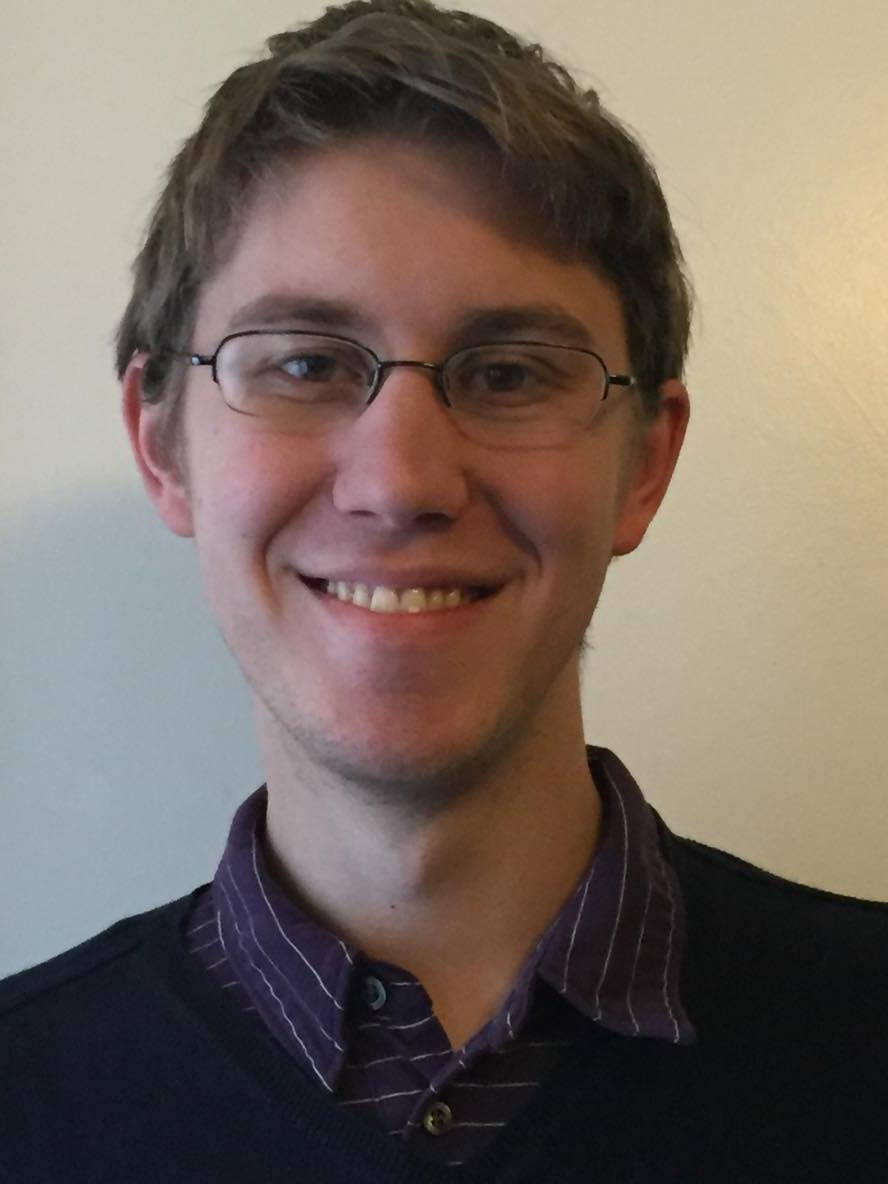
\includegraphics[width=1in,height=1.25in,clip,keepaspectratio]{biography/bart}}]{Austin Cory Bart} (Member, IEEE) received his PhD at Virginia Tech in Computer Science along with a certification in Learning Sciences. He received his undergraduate degree from the University of Delaware in Computer Science. His research interests are Computer Science Education, Software Engineering, and Program Analysis.
\end{IEEEbiography}

\begin{IEEEbiography}[{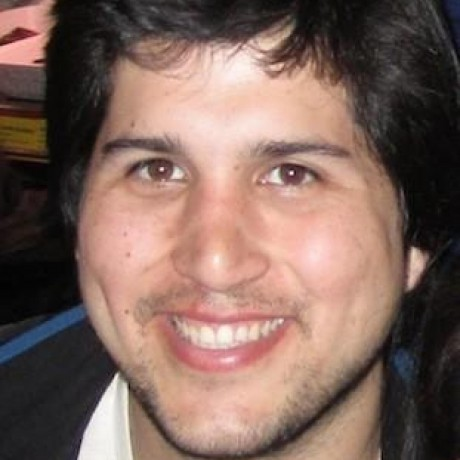
\includegraphics[width=1in,height=1.25in,clip,keepaspectratio]{biography/tibau}}]{Javier Tibau} (Member, IEEE) is a PhD candidate at Virginia Tech studying Computer Science. He is also an Assistant Professor at Escuela Superior Politecnica del Litoral (ESPOL). His research interests are in Human-Computer Interaction, and Computer Science Education.
\end{IEEEbiography}

\begin{IEEEbiography}[{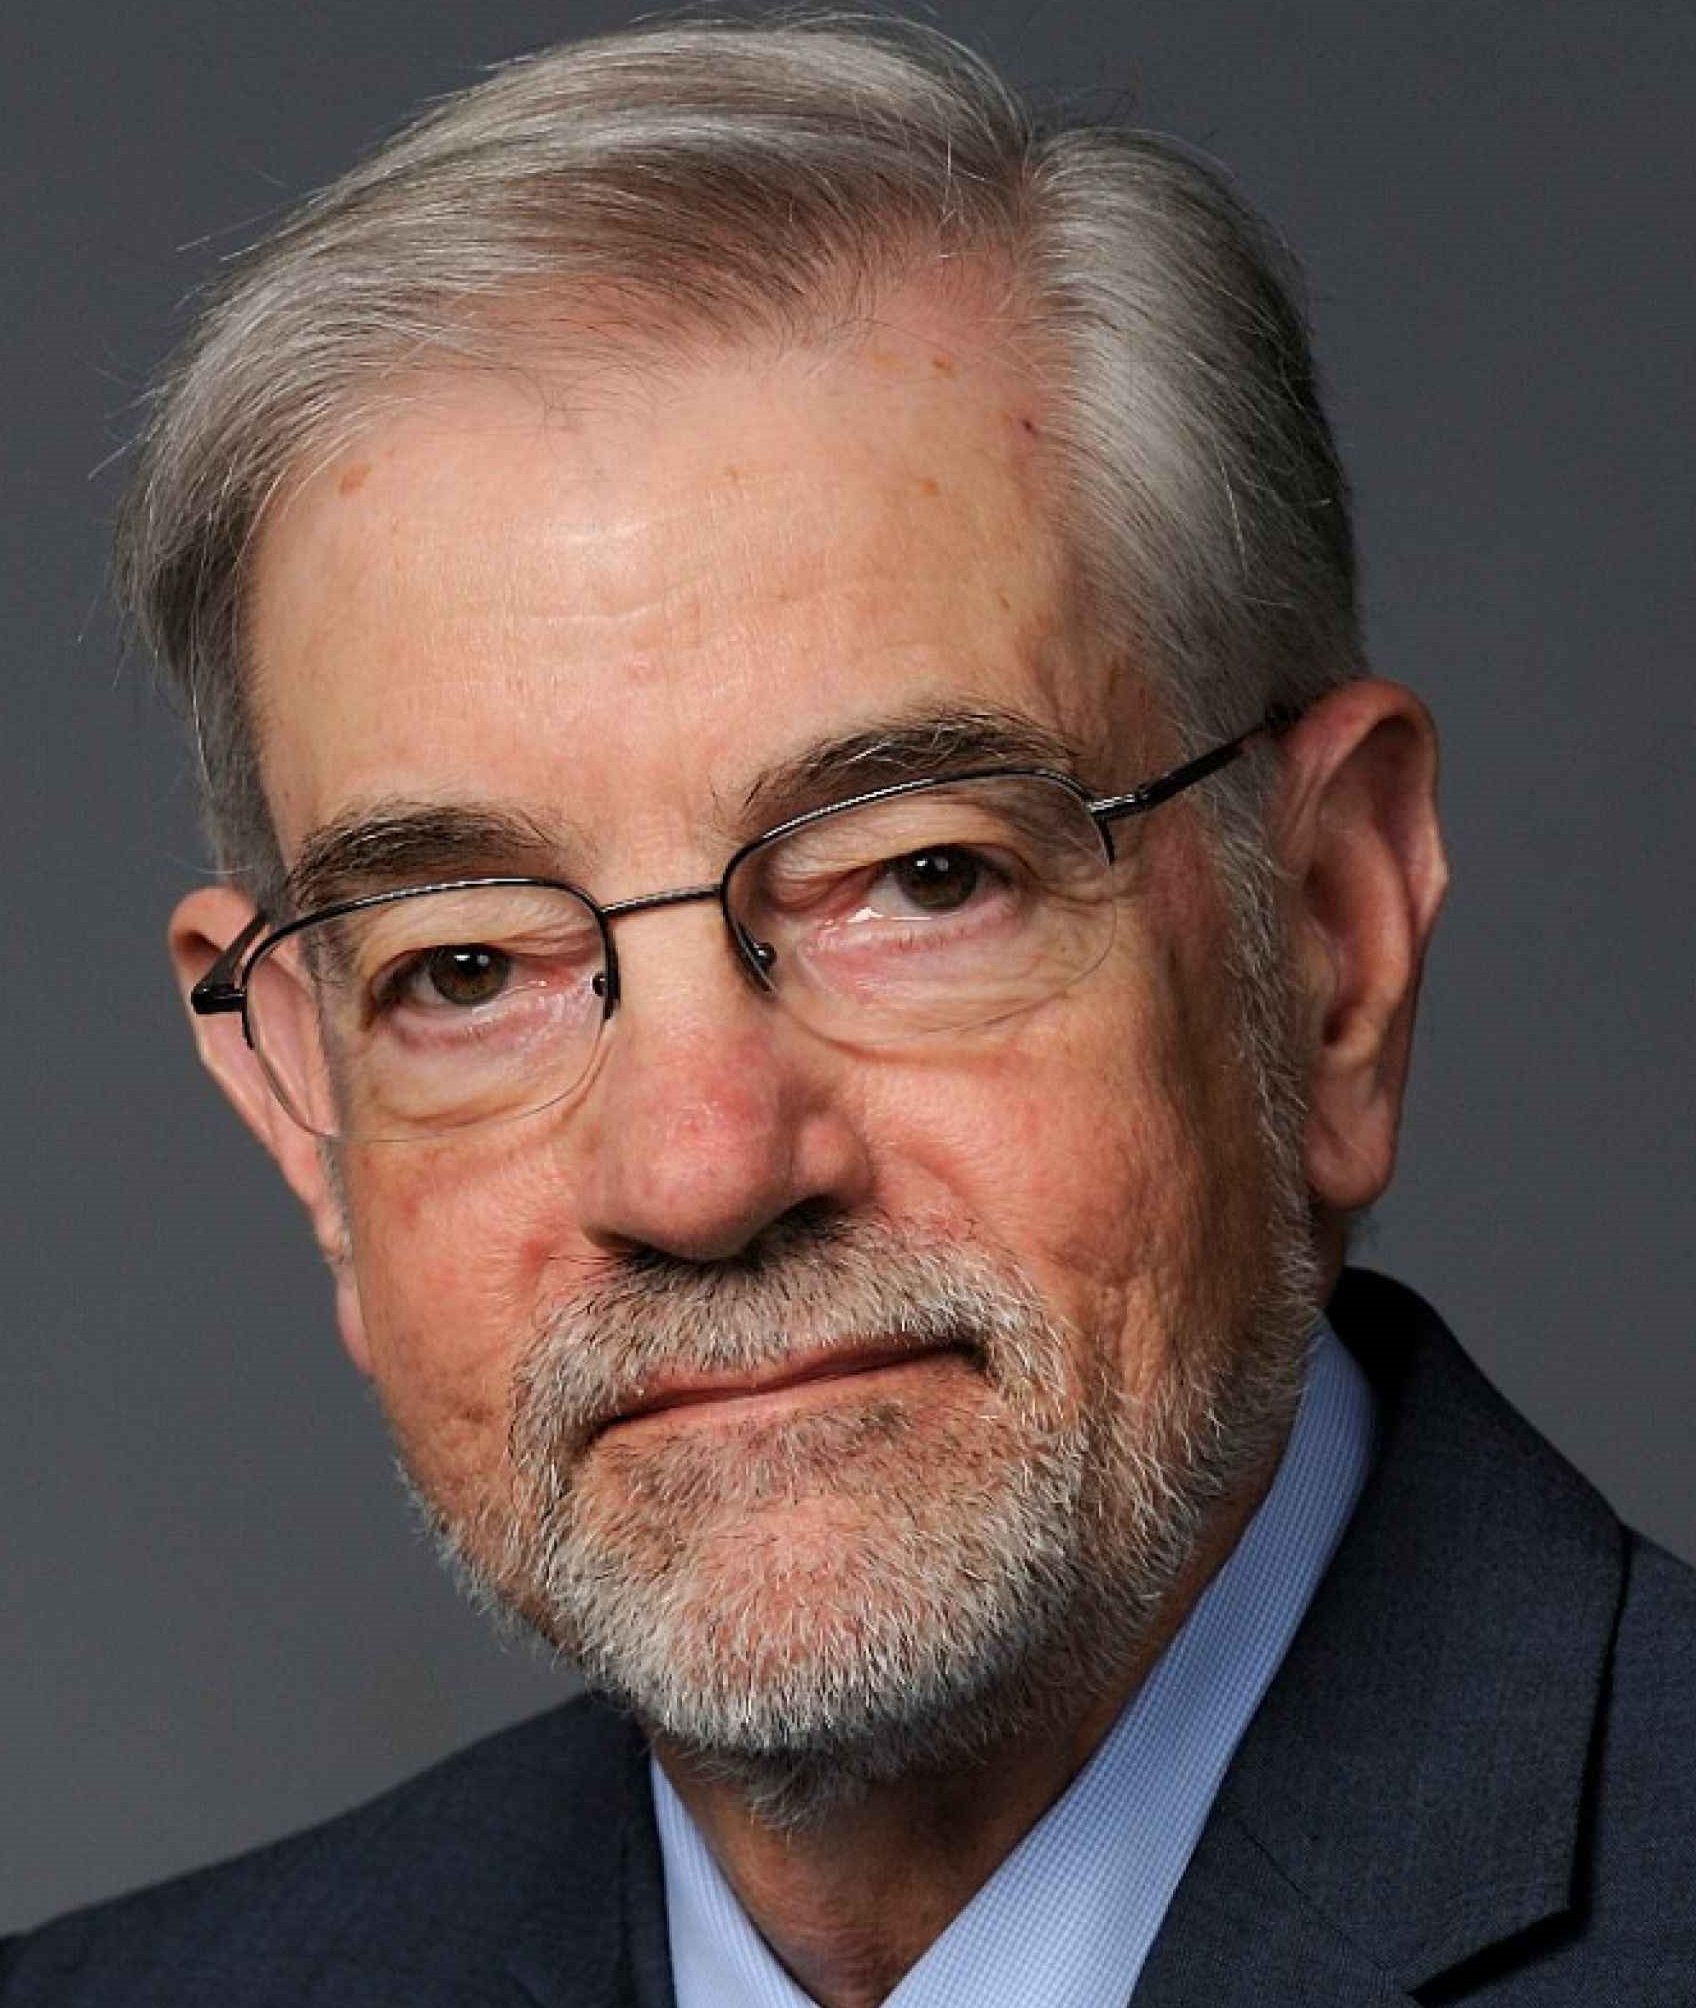
\includegraphics[width=1in,height=1.25in,clip,keepaspectratio]{biography/kafura}}]{Dennis Kafura} (Member, IEEE) received his PhD from Purdue University. He is a Professor of Computer Science at Virginia Tech. He is the PI on two NSF IUSE awards both of which involved the development of a general education course in Computational Thinking at the university level using the BlockPy environment.
\end{IEEEbiography}

\begin{IEEEbiography}[{
\includegraphics[width=1in,height=1.25in,clip,keepaspectratio]{biography/shaffer}}]{Clifford A. Shaffer} (Senior Member, IEEE and Distinguished Member, ACM) received his PhD from the University of Maryland.
He is Professor of Computer Science at Virginia Tech.
His current research interests are in Computational Biology (specifically, user interfaces for specifying models and computations), Algorithm Visualization, and Computer Science Education.

\end{IEEEbiography}

\begin{IEEEbiography}[{
\includegraphics[width=1in,height=1.25in,clip,keepaspectratio]{biography/tilevich}}]{Eli Tilevich}(Senior Member, IEEE) received his PhD from Georgia Tech.
He is an Associate Professor of Computer Science at Virginia Tech. His recent publications and current research focus on Software Engineering for Distributed and Mobile Computing and on Computer Science Education.
\end{IEEEbiography}


% that's all folks
\end{document}


